\documentclass[14pt,a4paper]{article}

\usepackage[a4paper, total={20cm, 27cm}]{geometry}

\usepackage[utf8]{inputenc}
\usepackage[T2A]{fontenc}
\usepackage[english,russian]{babel}
\usepackage{cmap}

\usepackage{amsmath, amssymb, amsfonts, amsthm, mathtools}
%\usepackage{microtype}
%\usepackage{lipsum}

\usepackage{graphicx}
\usepackage{sectsty}
\usepackage{xcolor}


\sectionfont{\fontsize{18}{14}\selectfont}
\subsectionfont{\fontsize{14}{14}\selectfont}
\renewcommand{\thesection}{\Roman{section}}
\renewcommand{\thesubsection}{\arabic{subsection}}

\graphicspath{{./images/}}

\title{\fontsize{26}{14}\selectfont\textbf{Вступительный экзамен в аспирантуру \\ 27.06.01}}
\author{Kirill Artemov \\ kaartemov@gmail.com}
\date{July 2018}

%%%%%%%%%%%%%%%%%%%%%%%%%%%%%%%%%%%%
\begin{document}
\maketitle

\section*{\centering РАЗДЕЛ I. Модели объектов управления}
\section{Описание прототипа}\label{prototype}

В описании к авторскому свидетельству №844986, кл. G 01 B 7/06 (по заявке №4822394/28 от 22.03.90 г., автор В.Г.Панов) представлено устройство \glqq Емкостной датчик микроперемещений\grqq, функциональная схема которого приведена на рисунке~\ref{schema}.

\begin{figure}[h]
	\centering
	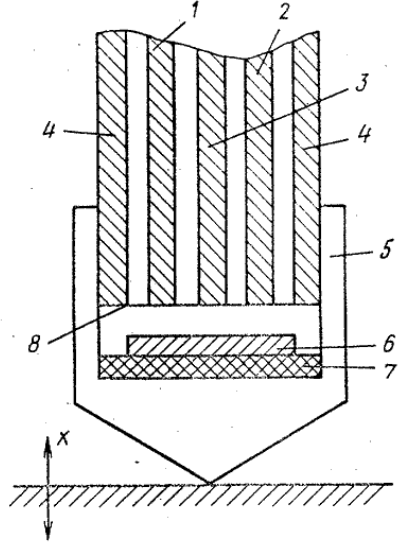
\includegraphics[width=0.4\textwidth]{schema.png}
	\caption{Функциональная схема датчика}
	\label{schema}
\end{figure}

Датчик содержит неподвижные потенциальный $1$ и измерительный $2$ электроды и охватывающие их внутренний $3$ и внешний $4$ экраны. Торцы электродов и экранов лежат в рабочей плоскости датчика. Снаружи боковой цилиндрической поверхности внешнего экрана $4$ размещен с возможностью возвратно- поступательного движения щуп $5$, во внутренней полости которого размещена металлическая пластина $6$, которая электрически изолирована от корпуса датчика и расположена параллельно рабочей плоскости его электродов и экранов. При перемещении щупа $5$ изменяется зазор между пластиной $6$ и рабочими торцами электродов и экранов, что приводит к изменению емкости датчика.

Датчик работает следующим образом: при перемещении объекта изменяется воздушный зазор между плоскостью металлической пластинки $5$ и рабочей плоскостью $8$ 
электродов $1$ и $2$ и экранов $3$ и $4$ датчика, вследствие чего изменяется выходное напряжение $U_{\text{вых}}$, снимаемое с измерительного электрода $2$ датчика. Чувствительность датчика зависит от величины диэлектрической постоянной материала контролируемого объекта и максимальна в диапазоне $0 - x_{\text{мин}}$, где $x_{\text{мин}}$~-- величина микроперемещения, когда металлическая пластина $6$ не заземлена. Герметизация щупа $5$ позволяет свести к минимуму погрешности, связанные с влиянием внешних условий.


\begin{figure}[h]
	\centering
	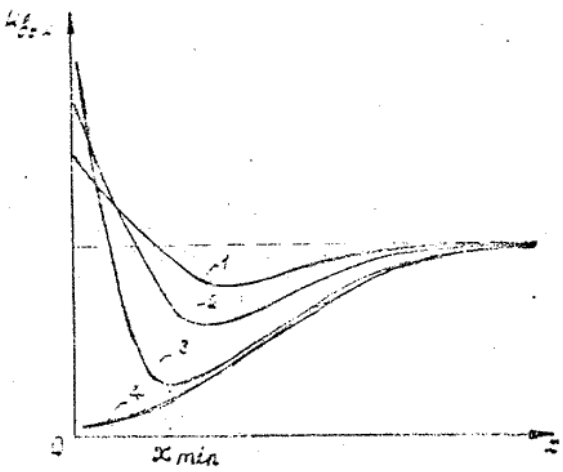
\includegraphics[width=0.4\textwidth]{out.png}
	\caption{Выходная характеристика в зависимости от диэлектрической проницаемости}
	\label{out}
\end{figure}


\section{Анализ и синтез по закону полноты частей системы}

%рабочий орган -- величина емкости между электродами и пластиной.
%трансмиссия -- пластина 6, подложка 7.
%двигатель -- щуп 7.

Определим основные части системы, представленной на рисунке~\ref{schema}. Сначала, определим рабочий орган -- Ро. Датчик предназначен для измерения расстояния. Расстояние выражается в изменении емкости между рабочей плоскостью 8 и пластиной 6. Изменение емкости влияет на выходное напряжение, которое измеряется при помощи с "конденсатора", образованного следующими элементами потенциальным электродом 1, пластиной 6 и измерительным электродом 2. 

Далее определим двигатель как часть системы, вырабатывающей энергетику. Здесь двигателем является балка, в которую упирается щуп 5. Тогда трансмиссией являются щуп, подложка 7 и пластина 6. Органов управления в рассматриваемом датчике нет, поэтому система является неполной. Структурная схема представлена на рисунке~\ref{first_sys}

\begin{figure}[h]
	\centering
	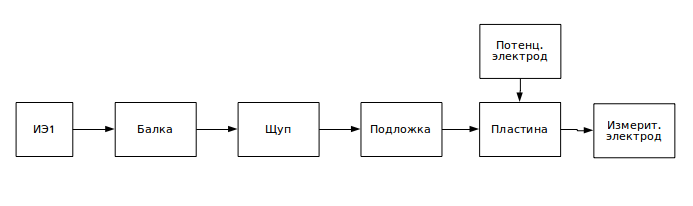
\includegraphics[width=1\textwidth]{pic0.png}
	\caption{Структурная схема рассматриваемой системы}
	\label{first_sys}
\end{figure}

Чтобы получить новые технические решения с использованием закона полноты частей  системы, можно добавить недостающие элементы в систему. 

Каждая ТС должна включать четыре части: двигатель, трансмиссию, рабочий орган и орган управления. Для синтеза ТС необходимо наличие этих четырех частей и их минимальная пригодность к выполнению функций системы.

Добавим в систему орган управления (ОУ).

Добавим в систему измерительную часть -- мостовую схему измерения, представленную на рисунке~\ref{im:bridge}, где $C_x$~-- представление датчика, как переменный конденсатор, $R_1$ и $R_2$~-- резисторы, У~-- усилитель, ИБ~-- измерительный прибор. Переменный конденсатор $C_3$, при помощи которого сможем подстраивать нулевое положения датчика. Этот конденсатор будет выступать в качестве Органа управления.


\begin{figure}[h]
	\centering
	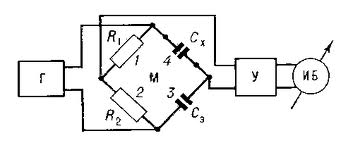
\includegraphics[width=0.6\textwidth]{bridge.jpg}
	\caption{Схема измерения емкости датчика с подстройкой}
	\label{im:bridge}
\end{figure}


\begin{figure}[h!]
	\centering
	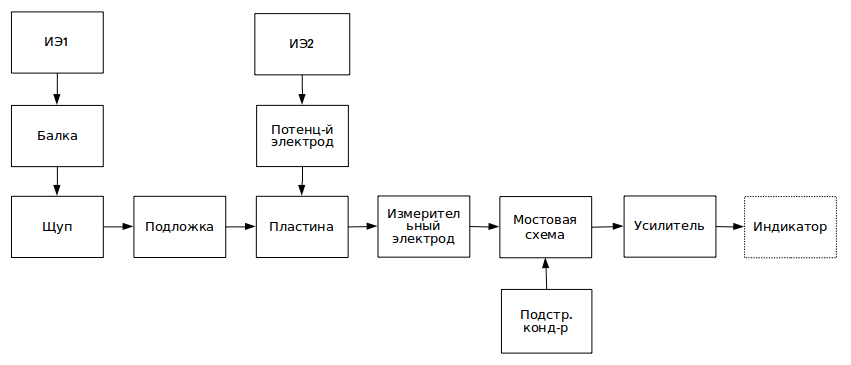
\includegraphics[width=1\textwidth]{pic1.png}
	\caption{Структурная схема полной системы}
	\label{pic1}
\end{figure}

Чтобы получить новые технические решения с использованием закона полноты частей системы, можно использовать линию на вытеснение человека из ТС. В соответствии с
линией вытеснения действия человека необходимо искать на окончании этой линии -- в органах управления.

В рассматриваемой системе балка давит на щуп, который в свою очередь это давление передает через подложку 7 на пластину 6. Пластина шесть изменяет свое положение относительно плоскости электродов 8. Электроды и пластина, образующие конденсатор, емкость которого изменяется, в результате чего с измерительной схемы на усилитель передается отклонение пластины от нулевого положения, заданного человеком при помощи подстроечного конденсатора. Для вытеснения этой функции человека этот конденсатор должен подстраиваться автоматически при включении системы. Нужно заменить конденсатор на устройство подстройки емкости, при помощи подачи некоторого информационного сигнала 
с надсистемы.

Система получается с автоматической калибровкой. Такая система обладает меньшими ошибками и более простой в использовании. 

Таким образом, с точки зрения закона получили полную систему.


\subsection{Анализ и синтез по закону энергетической и информационной проводимости ТС}


Необходимым условием принципиальной жизнеспособности ТС является сквозной проход энергии и информации по всем частям технической системы. 

Проанализируем систему с рисунка~\ref{pic1} по закону энергетической проводимости. Построение линии начнем с ИП, рисунок~\ref{im:bridge}, он выделяет электрическую энергию. Электрическое поле ИП воздействие на потенциальный электрод, на выходе которого формируется напряжение. Информативный параметр электрического поля в данном случае -- это переменное напряжения. 
Поле давления действует на щуп, в результате чего он изменяет свое положение относительно корпуса. 
Поле давления от щупа воздействует на подложке. Поле давления от подложки воздействует на пластину. Электрическое поле от потенциального электрода воздействует на пластину. Электрическое поле от пластины воздействует на измерительный электрод. Электрическое поле от Измерительного электрода воздействует на Мостовую измерительную схему. Информационным параметр электрического поля в этом случае -- это рассогласование емкости эталонного конденсатора и емкости между электродами и пластиной. Поле электрического поля от мостовая схемы воздействует на усилитель. Выходным информационным параметром усилителя будет напряжение.


\begin{figure}[h!]
	\centering
	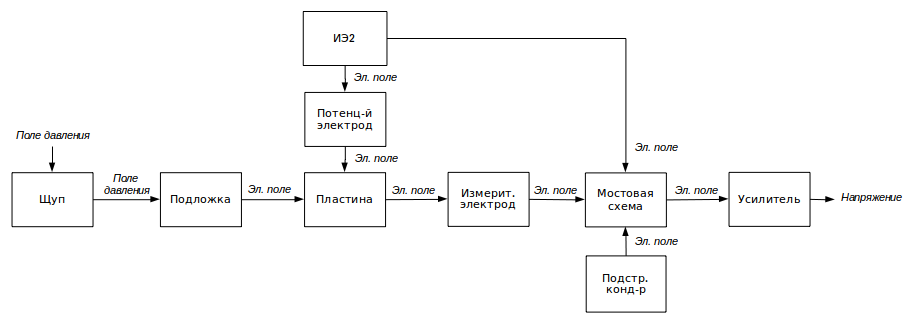
\includegraphics[width=1\textwidth]{pic2.png}
	\caption{Линия прохода энергии и информации}
	\label{}
\end{figure}

Для синтеза новых решений можно замкнуть линию прохождения энергии, получив кольцо. 

По этому закону можно дополнить систему на входе регулятором и пьезодвигателем, поле давление которого будет воздействовать на щуп. Для этого выход усилителя замкнем на вход регулятора, напряжение которого будем подавать на пьезодвигатель.

\begin{figure}[h!]
	\centering
	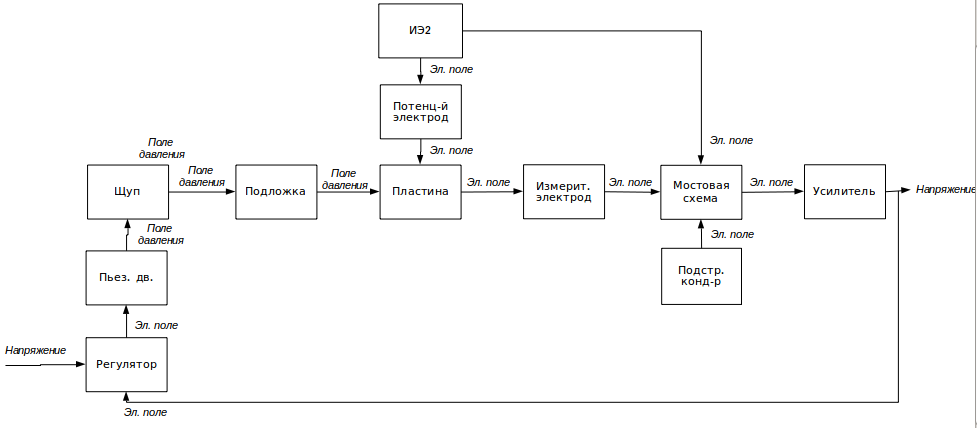
\includegraphics[width=1\textwidth]{pic3.png}
	\caption{Линия прохода энергии и информации с замкнутой схеме}
	\label{sogl}
\end{figure}

\section{Закон согласования-рассогласования технических систем}

Составляющие техническую систему части должны быть согласованы или, наоборот, рассогласованы между собой.

С точки зрения этого закона можно проверить согласованность по темпам протекания процессов, происходящих в основных частях системы.

Система рассогласована по темпам протекания процессов. Изменение расстояния между пластиной и плоскостью электродов, происходит медленнее, чем протекают токи в электрических схемах мостовой схемы и усилителя. Чтобы согласовать ее, можно заменить электрическую часть механической, в которой перемещение щупа через механические передачи будет преобразовываться в показания стрелочного индикатора.

С точки зрения энергетических параметром, полученная система на рисунке~\real{sogl} согласована по входным и выходным информационным сигналам.

Система рассогласована в части параметров материалов. Для согласования системы, чтобы избавиться от вредного явления трения между корпусом и щупом, а в перспективе и износа щупа, можно убрать щуп.

Рисунок с механическим измерением

\section{Анализ и синтез систем по закону увеличения степени идеальности}

Закон увеличения степени идеальности является одним из основных законом развития ТС. Под увеличением степени идеальности И в ТРИЗ понимается рост отношения суммы выполняемых системой полезных функций Фп к сумме факторов расплаты Фр.



%Для повышения степени идеальности путем увеличения числителя формулы необходимо возложить на систему еще одну или несколько функций, ранее ею не выполнявшихся. Например, при добавлении обратной связи, позволяющей стабилизировать конструкцию в зависимости от выходного напряжения можно получить новое устройство - стабилизирующая платформа. Факторами расплаты в этом случае будут являться добавление новых элементов в систему, таких как двигатель и редуктор.

%При добавлении датчиков, сигнализирующих о достижении крайнего положения отклонения, например герконов, получим еще одну функцию системы – контроль достижения предельного отклонения.

%Рисунок 6 – Использование датчиков крайнего положения

%Попробуем уменьшить знаменатель. Для этого исключим из системы какую-либо её часть, например элемент масштабирования. Измерение отклонения проводить по прежнему можно, но это уменьшит точность.

\section{Закон неравномерного развития технических систем}

%;ехнической системы появляются противоречия, происходит накопление и обострение противоречий.

%Выберем содержательную характеристику, которую будем улучшать.

%Для данного датчика выберем повышение чувствительности. Если отклонить конструкцию на очень малый угол, то на выходе катушек 4, 6 индуктивности не появляется напряжение, достаточное для формирования выходного сигнала.

%Чем тяжелее маятник, тем точнее будет измерение. Но увеличивается размер и тем самым деформируется шарнир. Возникает противоречие: маятник должен быть большим для увеличения точности и не большим, чтобы он не деформировал шарнир.

%Разрешим это противоречие с помощью алгоритма решения изобретательских задач (АРИЗ).

\newpage
\subsection{Понятие передаточной функции и передаточной матрицы непрерывных систем}

Переда́точная функция~--- один из способов математического описания динамической системы. Представляет собой дифференциальный оператор, выражающий связь между входом и выходом линейной стационарной системы. Зная входной сигнал системы и передаточную функцию, можно восстановить выходной сигнал.

Например, для линейной модели ВВ одноканального объекта управления:
\begin{equation}
    a(p) y(t) = b(p) u(t),
\end{equation}
передаточкая фукция будет иметь вид:
\begin{equation}
    y(t) = \cfrac{b(p)}{a(p)} u(t) = W(p) u(t),
\end{equation}
где $W(p)$~--- интегралльно--дфифференциальный опрератор или передаточная функция, $a_i, b_i$~--- параметры модели, $n$~--- порядок модели, $r = n - m \ge 1$~--- относительная степень модели. В физически реализуемых системах относительная степень модели не должна быть меньшей единицы.


В случае $u(t)=0$ система называется автономной. $a(p)=0$~--- характеристический полином, где его корни $p_i$~--- полюсы системы. $b(p)=0$~--- характеристический полином правой части, где его корни $p_i^0$~--- нули системы. В случае $a_0 = 1$~--- характеристический полином называется приведенным.

Преимущество использования таких операторных моделей: краткость записи уравнений; удобство преобразования сложных моделей.

Для MIMO-систем вводится понятие \textbf{матричной передаточной функции}. 
Если для системы
\begin{equation}
    \dot x = A x + b u, \quad y = C x
\end{equation}
для нулевых начальных условий и при $p = d/dt$ записать:
\begin{equation}
    x = (p I - A)^{-1} B \cdot u \quad\Rightarrow\quad y = C(p I - A)^{-1} B \cdot u,
\end{equation}
то получим передаточную матрицу системы 
\begin{equation}
    W(p) = C(p I - A)^{-1}.
\end{equation}
где $(p I - A)^{-1}$~--- резольвента, которую можно переписать в виде:
\begin{equation}
    (p I - A)^{-1} = \cfrac{adj(pI - A)}{det(pI - A)} = \cfrac{p^{n-1} + R_1 p^{n-2} + \dots + R_n}{det(pI - A)}
\end{equation}
где характеристический полином системы:
\begin{equation}
    det(pI - A) = a(p)
\end{equation}
где собственные числа матрица $A$ в точности совпадают с полюсами системы $\lambda_i\{A\} = p_i$.

В матрица $W(p)$ на месте $ij$ элемента стоит обычная передаточная функция от $i$-ого входа к $j$-у выходу.


\subsection{Понятия структурных схем и структурных преобразований}
Структурная схема~--- это графическое изображение системы в виде блоков с передаточными функциями и связей между ними. На схемах указываеются входныя, промежуточные и выходные переменные.

Структурная схема САУ в простейшем случае строится из элементарных динамических звеньев. Но несколько элементарных звеньев могут быть заменены одним звеном со сложной передаточной функцией. Для этого существуют правила эквивалентного преобразования структурных схем. Рассмотрим возможные способы преобразований для трех элементарных звеньев:
\begin{equation}
    y_1 = W_1 x_1, \quad y_2 = W_2 x_2, \quad y_3 = W_3 x_3.
\end{equation}
\begin{enumerate}
    \item Последовательное соединение:
    \begin{figure}[h!]
        \begin{minipage}[h]{0.5\linewidth}
            \centering{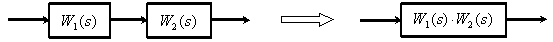
\includegraphics[width=0.5\linewidth]{images/serial.png}}
        \end{minipage}
        \begin{minipage}[h]{0.5\linewidth}
            \begin{equation}
                y = W_1 W_2 W_3 x
            \end{equation}
        \end{minipage}
    \end{figure}
    
    \item Параллельное соединение:
    \begin{figure}[h!]
        \begin{minipage}[h]{0.5\linewidth}
            \centering{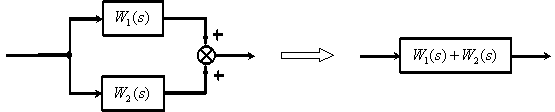
\includegraphics[width=0.5\linewidth]{images/parallel.png}}
        \end{minipage}
        \begin{minipage}[h]{0.5\linewidth}
            \begin{equation}
                y = (W_1 + W_2 + W_3) x
            \end{equation}
    \end{minipage}
    \end{figure}
    
    \item Замкнутая система с ООС (ОС~--- $W_3$):
    \begin{figure}[h!]
        \begin{minipage}[h]{0.5\linewidth}
            \centering{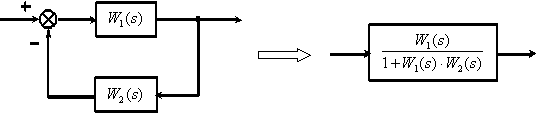
\includegraphics[width=0.5\linewidth]{images/ooc.png}}
        \end{minipage}
        \begin{minipage}[h]{0.5\linewidth}
            \begin{equation}
                y = \cfrac{W_1 W_2}{1 + W_1 W_2 W_3} x
            \end{equation}
        \end{minipage}
    \end{figure}

    \item Замкнутая система с ПОС (ОС~--- $W_3$):
    \begin{figure}[h!]
        \begin{minipage}[h]{0.5\linewidth}
            \centering{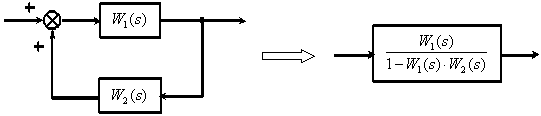
\includegraphics[width=0.5\linewidth]{images/poc.png}}
        \end{minipage}
        \begin{minipage}[h]{0.5\linewidth}
            \begin{equation}
                y = \cfrac{W_1 W_2}{1 - W_1 W_2 W_3} x
            \end{equation}
        \end{minipage}
    \end{figure}
    
    \item Перенос точки ветвления через динамическое звено:
    \begin{figure}[h!]
        \begin{minipage}[h]{0.5\linewidth}
            \centering{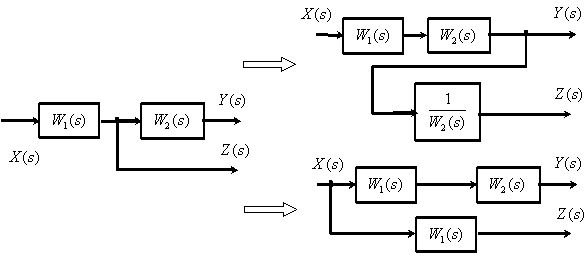
\includegraphics[width=0.5\linewidth]{images/transfer_point.png}}
        \end{minipage}
        \begin{minipage}[h]{0.5\linewidth}
            \begin{gather}
                y = W_1 W_2 x, \\
                z_{fwd} = W_1 W_2 \cfrac{1}{W_2}, \\
                z_{bwd} = W_1
            \end{gather}
        \end{minipage}
    \end{figure}
    
    \item Перенос суммирующего звена через динамическое звено:
    \begin{figure}[h!]
        \begin{minipage}[h]{0.5\linewidth}
            \centering{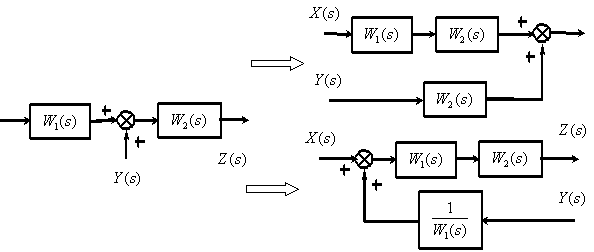
\includegraphics[width=0.5\linewidth]{images/transfer_sum.png}}
        \end{minipage}
        \begin{minipage}[h]{0.5\linewidth}
            \begin{gather}
                z = (W_1+W_2 y) x, \\
                z_{fwd} = W_1 W_2 x + W_2 y, \\
                z_{bwd} = W_1 W_2 (\cfrac{1}{W_2}y + x)
            \end{gather}
        \end{minipage}
    \end{figure}    
\end{enumerate}
    
\subsection{Аппарат частотных характеристик систем управления: амплитудно-фазовые 	характеристики; амплитудная и фазовая частотные характеристики и логарифмические 	амплитудно-фазовые частотные характеристики}

Различают два вида характеристик САУ и их звеньев: временные и частотные.

Временные характеристики (переходная, весовая) получают подавая на вход СУ эталонные сигналы: $\mathbf{1}(t), \delta(t)$. 

Частотные характеристики СУ и их звеньев получаются рассмотрением вынужденных движений системы (звена) при подаче на ее вход гармонического сигнала:
\begin{equation}
    x(t) = A \sin{\omega t},
\end{equation}
где $\omega$~--- частота.

При таком входе на выходе линейной системы в установившемся режиме (при больших $t$) будет синус той же частоты (для устойчивых систем), но с другой амплитудой $A$ и сдвигом фазы $\phi$:
\begin{equation}
    x(t) = A(\omega) \sin{(\omega t + \phi(\omega))}.
\end{equation}

Зная ПФ СУ можно вычислить амплитуду и сдвиг фазы:
\begin{equation}
    A(\omega) = |\W(j \omega)|, \quad \phi(\omega) = \arg{W(j \omega)} = \arctan{\cfrac{Im W(j \omega)}{Re W(j \omega)}}.
\end{equation}
где $j \omega = s$, т.е. в обычную ПФ вместо $s$ подставляется только мнимая ее часть.
Для кажой частсоты $\omega$ значение $W(j \omega) = P + jQ = A(\omega) e^{-j\phi(\omega)}$~--- это некторое комплексное число с амплитудой $|W(j \omega)| = \sqrt{P^2 + Q^2}$ и фазой $\arg W(j \omega) = \arctan{\cfrac{Q}{P}}$. 

ПФ $W(j \omega$~--- называется \textbf{частотной характеристикой звена}, т.к она характеризует выход системы при гармонических сигналах разной частоты. Где $P, Q$~--- вещественная и мнимая частотные характеристики.

Функции $A(\oemga), \phi(\omega)$~--- называются соответственно \textbf{амплитудной и фазовой характеристиками} (АЧХ и ФЧХ). \textit{Амплитудная характеристика}~--- это коэффициент усиления гармонического сигнала.

По форме АЧХ различают несколько основных типов звеньев:
\begin{enumerate}
    \item ФНЧ~--- пропускает низкочастотные сигналы примерно с одинаковым коэффициентом усиления, ослабляет высокочистотные шумы и помехи;
    \item ФВЧ~--- пропускает высокие, ослаблляет низкие;
    \item полосовой фильтр~--- комбинация предыдущих;
    \item полосовой режекторный фильтр~--- инвертированные предыдущий.
\end{enumerate}

\textbf{Амплитудно-фазовая частотная характеристика} (АФЧХ) — удобное представление частотного отклика линейной стационарной динамической системы в виде графика в комплексных координатах.

На комплексной плоскости $W$ (см. рисунок) комплексное число  изображается вектором ОС, длина которого равна $A(\omega)$, а аргумент это угол $\phi(\omega)$ образованный этим вектором с действительной положительной полуосью.

При изменении частоты от 0 до $\infty$ вектора ОС (точка) опишет некоторую кривую, которая называется годографом амплитудно-фазо-частотной характеристики.

\begin{figure}[h!]
    \begin{minipage}[h]{0.5\linewidth}
        \centering
        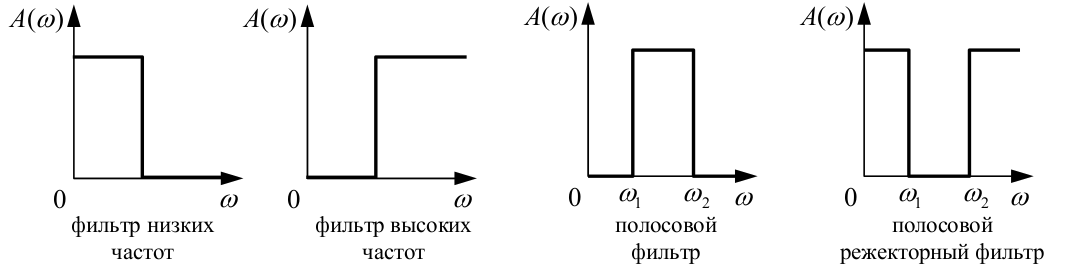
\includegraphics[width=0.8\linewidth]{images/af.png}
        \caption{Амплитудные характеристики идеальных фильтров}
        \label{fig:a_filters}    
    \end{minipage}
    \begin{minipage}[h]{0.5\linewidth}
        \centering
        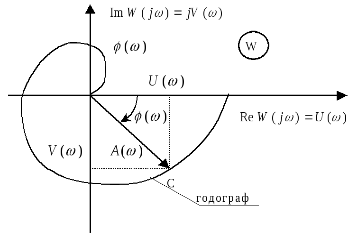
\includegraphics[width=0.5\linewidth]{images/aphf.png}
        \caption{АФЧХ}
        \label{fig:aphf}
    \end{minipage}
\end{figure}
В практике исследований систем автоматического управления широко применяются логарифмические амплитудно-частотные и фазо-частотные характеристики.

Частотные характеристики достаточно сложно строить вручную. В 60-е годы, когда раз вивалась классическая теория управления, не было мощных компьютеров, поэтому наибольшую популярность приобрели приближенные методы, с помощью которых можно было проектировать регуляторы с помощью ручных вычислений и построений. Один из таких подходов основа на использовании логарифмических частотных характеристик. 
Вместо $A(\oemga)$ было предложено использовать логарифмическую амплитудную частотных характеристику (ЛАЧХ): график, на котором по оси абсцисс откладывается десятичный лога рифм частоты $(\log\omega)$, а по оси ординат~--- величина, измеряемая в децибелах (дБ). При построении логарифмической фазовой частотной характеристики (ЛФЧХ) по оси абсцисс также откладывается логарифм частоты. Единицей отсчета на логарифмической оси частот является декада~--- диапазон, на котором частота увеличивается в 10 раз (а значение ее логарифма увеличивается на единицу). Вместе ЛАЧХ и ЛФЧХ называются логарифмической амплитудно-фазовой частотной характеристикой (ЛАФЧХ) или диаграммой Боде.

\textbf{Логарифмическая амплитудно-частотная} ЛАЧХ характеристика системы автоматического управления~--- это кривая, cоответствующая двадцати десятичным логарифмам модуля $W(j \oemga)$, построенной в десятичном логарифмическом масштабе частот~--- размерность децибел. ЛАЧФ:
\begin{equation}
    L(\omega) = 20 \log{|W(j \omega)|} = 20 \log{A(\omega)}
\end{equation}

\textbf{Логарифмическая фазо-частотная характеристика} ЛФЧХ системы автоматического управления~--- это её фазо-частотная характеристика $\phi(\omega)$, построенная в логарифмическом масштабе частот.

Ценность частотных характеристик состоит в том, что они позволяют косвенно судить о процессах, происходящих в системах автоматического управления (не решая дифференциальных уравнений, описывающих данную систему).

Для построения логарифмической амплитудно-частотной характеристики принято брать более мелкую единицу измерения, которая в 20 раз меньше одной десятичной логарифмической единицы

В ЛЧХ единица измерения ординат~--- децибел, по оси абсцисс~--- декада. Частота, для которой $A(\oemga_c) = 1$~--- называется частотой среза. Для устойчивых система значение фазына частоте среза должно быть больше $-180^o$, а годограф не должен охватывать точку $(-1, 0)$.















\subsection{Типовые звенья непрерывных систем, частотные характеристики типовых звеньев}

Обычно система управления состоит из отдельных блоков, каждый из которых описывается уравнениями низкого порядка (первого и второго). Для понимания работы системы в целом желательно хорошо представлять, как ведут себя ее отдельные элементы. Для построения ЛАФЧХ передаточную функцию системы зазбивают на простейшие сомножители и строят характеристику для всей системы как сумму  ЛАЧХ и ЛФЧХ отдельных звеньев.

\begin{enumerate}
    \item Пропорциональное (безъинерционное) звено
    \begin{figure}[!h]
        \begin{minipage}[!h]{0.5\linewidth}
            \centering{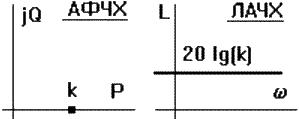
\includegraphics[width=1\linewidth]{images/links/pl.png}}
        \end{minipage}
        \begin{minipage}[!h]{0.5\linewidth}
            \begin{gather}
                W(s) = k, \quad W(j \omega) = k, \quad k \ne 0, \\
                \text{AЧХ и ФЧХ:\:\:}
                A(\omega) = k, \quad \phi(\omega) = 0, \\
                \text{ЛАФЧХ:\:\:}
                \begin{cases}
                    L(\omega) = 20 \log k \\
                    \phi(\omega) = 0.
                \end{cases}
            \end{gather}
        \end{minipage}
    \end{figure}

    \item Апериодическое звено
    \begin{figure}[!h]
        \begin{minipage}[!h]{0.5\linewidth}
            \centering{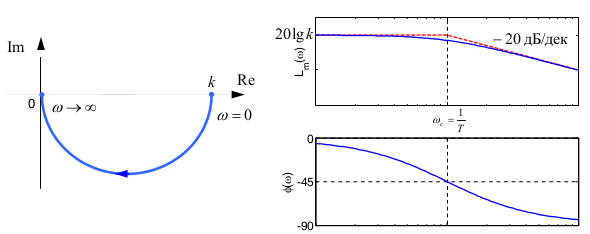
\includegraphics[width=1\linewidth]{images/links/al.png}}
        \end{minipage}
        \begin{minipage}[!h]{0.5\linewidth}
            \begin{gather}
                W(s) = \cfrac{k}{Ts + 1} = \cfrac{k - j k T \omega}{T^2 \omega^2 + 1}, \quad k \ne 0, T > 0 \\
                \text{AЧХ и ФЧХ:\:\:}
                A(\omega) = \cfrac{k}{\sqrt{T^2 \omega^2 + 1}}, \\ 
                \phi(\omega) = \arctan{\cfrac{ImW}{ReW}} = -\arctan{T \omega}, \\
                \text{ЛАФЧХ:\:\:}
                \begin{cases}
                    L(\omega) = 20 \log A(\omega) = -20 \log \sqrt{1+T^2 \omega^2} \\
                    \phi(\omega) = -\arctan{T \omega}.
                \end{cases}
            \end{gather}
        \end{minipage}
    \end{figure}
    
    \item Интегрирующее звено
    \begin{figure}[!h]
        \begin{minipage}[!h]{0.5\linewidth}
            \centering{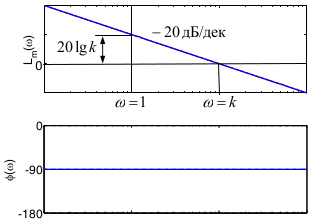
\includegraphics[width=1\linewidth]{images/links/il.png}}
        \end{minipage}
        \begin{minipage}[!h]{0.5\linewidth}
            \begin{gather}
                W(s) = \cfrac{k}{Ts} = \cfrac{k}{T j \omega}, \quad k \ne 0, T > 0 \\
                \text{AЧХ и ФЧХ:\:\:}
                A(\omega) = \cfrac{k}{T \omega}, \\ 
                \phi(\omega) = -\arctan{(-\infty)} = -\cfrac{\pi}{2}, \\
                \text{ЛАФЧХ:\:\:}
                \begin{cases}
                    L(\omega) = -20 \log T \omega \\
                    \phi(\omega) = -\cfrac{\pi}{2}.
                \end{cases}
            \end{gather}
        \end{minipage}
    \end{figure}
    
    \item Колебательное звено
    \begin{figure}[!h]
        \begin{minipage}[!h]{0.5\linewidth}
            \centering{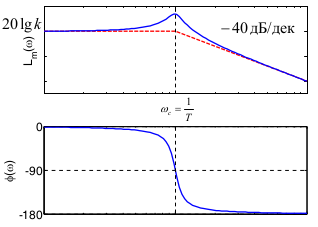
\includegraphics[width=1\linewidth]{images/links/gl.png}}
        \end{minipage}
        \begin{minipage}[!h]{0.5\linewidth}
            \begin{gather}
                W(s) = \cfrac{k}{T^2s^2 + 2 \xi T s + 1} = \cfrac{1-T^2\omega^2 - j 2 \xi T \omega}{4 \xi^2 T^2 \omega^2 + (1 - T^2 \omega^2)^2}, \\
                \text{AЧХ и ФЧХ:\:\:}
                A(\omega) = \cfrac{k}{\sqrt{4 \xi^2 T^2 \omega^2 + (1 - T^2 \omega^2)^2}}, \\ 
                \phi(\omega) = -\arctan{\cfrac{2 \xi T \omega}{1 - T^2 \omega^2}}, \\
                \text{ЛАФЧХ:\:\:}
                \begin{cases}
                    L(\omega) = -20 \log \sqrt{4 \xi^2 T^2 \omega^2 + (1 - T^2 \omega^2)^2} \\
                    \phi(\omega) = -\arctan{\cfrac{2 \xi T \omega}{1 - T^2 \omega^2}}.
                \end{cases}
            \end{gather}
        \end{minipage}
    \end{figure}
    
    \item Идеальное дифференцирующее звено
    \begin{figure}[!h]
        \begin{minipage}[!h]{0.5\linewidth}
            \centering{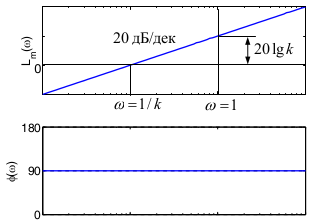
\includegraphics[width=1\linewidth]{images/links/dl.png}}
        \end{minipage}
        \begin{minipage}[!h]{0.5\linewidth}
            \begin{gather}
                W(s) = k s = k j \omega, \\
                \text{AЧХ и ФЧХ:\:\:}
                A(\omega) = k \omega, \\ 
                \phi(\omega) = \cfrac{\pi}{2}, \\
                \text{ЛАФЧХ:\:\:}
                \begin{cases}
                    L(\omega) = 20 \log(j k \omeg) \\
                    \phi(\omega) = \cfrac{\pi}{2}.
                \end{cases}
            \end{gather}
        \end{minipage}
    \end{figure}

\end{enumerate}



\subsection{Переходная и весовая функции непрерывной системы. Свободная, вынужденная, переходная и установившаяся составляющие движения непрерывной системы}

\textit{Переходным процессом} называют процесс изменения во вреени различных переенных системы (фазовых, выходных, отклонений и т.д.) в ходе которых система изменяет свое состояние.
Перехдные процессы могут быть представлены аналитически или графически.
К графическим можно отнести: временные диаграммы переменных системы ($y(t), \dot y(t), \dots$) и фазовые траектории.
Для аналитического представления нужно режать ДУ системы.

Решение $y(t)$ (или $y_{\text{п}}(t)$~--- переходная составляющая) может быть представлено в виде суммы свободной и вынужденной составляющих:
\begin{equation}
    y(t) = y_{\text{св}}(t) + y_{\text{в}}(t)
\end{equation}
где $y_{\text{в}}(t)$~--- вынужденная составляющая, соответствующая переходному процессу системы при нулевых начальных условиях $y_0^{(i)} = 0$ и явлается реакцией системы на входное воздействие $u(t)$,
$y_{\text{св}} (t)$~--- свободная составляющая или переходный процесс автономной системы, соответствует решениям ОДУ системы и зависит от начальных условий.

Свободная составляющая зависит от полюсов системы и определяется выражениями:
\begin{enumerate}
    \item Для попарно различных (некратных) корней:
    \begin{equation}
        y_{\text{св}} (t) = \sum\limits_{i=0}^{n} y_i(t) = \sum\limits_{i=0}^{n} C_i e^{p_i t},
    \end{equation}
    где $C_i e^{p_t t}$~--- свободные колебания системы или моды.
    \begin{enumerate}
        \item Вещественные корни $p_i = \alpha_i$ представляют апериадичускую составляющую:
        \begin{equation}
            y_i = C_i e^{\alpha_i t}.
        \end{equation}
        \item Пары комплексно-сопряженных коней $p_i = \alpha_i \pm j \beta_i$ колебательную составляющую:
        \begin{equation}
            y_{i, i+1} = A_i e^{\alpha_i t} \sin{(\beta_i t + \phi_i)}.
        \end{equation}
    \end{enumerate}
    \item Для кратных корней:
    \begin{equation}
        y_{i, i+1} = (C_i + C_{i+1} t) \cdot e^{\alpha_i t}
    \end{equation}
\end{enumerate}

Вынужденная составляющая переходного процесса зависит от входного воздействия и может быть аналитически определена только для ряда частных случаев, соответствующих некоторым типовым входным сигналам. Наиболее распространнеными сигналами являеются единичный скачек, дельта-функция и гармоничческое воздействие.
\begin{enumerate}
    \item Единичный скачек.
    \begin{figure}[!h]
        \begin{minipage}[!h]{0.5\linewidth}
            \centering{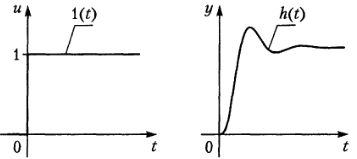
\includegraphics[width=0.8\linewidth]{images/input/1.png}}
        \end{minipage}
        \begin{minipage}[!h]{0.5\linewidth}
            \begin{equation}
                \mathbf{1}(t) = 
                \begin{cases}
                    0, for \: t \le 0, \\
                    1, for \: t > 0.
                \end{cases}
            \end{equation}
            Переходный процесс $y(t) = h(t)$ системы при ННУ и воздействии на ее вход ступенчатой единичной функции называется переходной функцией (характеристикой).
        \end{minipage}
    \end{figure}
    
    \item Дельта функция (единичная импульсная функция).
    \begin{figure}[!h]
        \begin{minipage}[!h]{0.5\linewidth}
            \centering{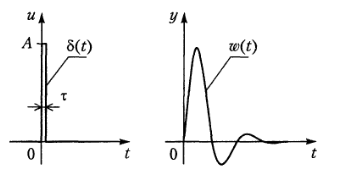
\includegraphics[width=0.8\linewidth]{images/input/delta.png}}
        \end{minipage}
        \begin{minipage}[!h]{0.5\linewidth}
            \begin{equation}
                \mathbf{\delta}(t) = \cfrac{d}{dt} \mathbf{1}(t).
            \end{equation}
            Переходный процесс $y(t) = w(t)$ системы при ННУ и воздействии на ее вход дельта-функции называется весовой функцией.
        \end{minipage}
    \end{figure}
\end{enumerate}

\textit{Установившейся режим}~--- это работа системы при $t \rightarrow \infty$:
\begin{equation}
    y_{\text{у}}(t) = \lim\limits_{t \rightarrow \infty} y_{\text{св}}(t)
    \quad\Rightarrow
    y(t) = y_{\text{п}}(t) + y_{\text{у}}(t)
\end{equation}

Если существуте предел (т.е. при достаточно больших t отсутствуют движения в системе)
\begin{equation}
    \lim\limits_{t \rightarrow \infty} y(t) = y_{\text{у}}(t),
\end{equation}
то такой режим называется статический режим работы системы.
\subsection{Понятие дискретных по времени объектов и систем, их математические модели}

Математические модели дискретных систем управления описывают поведение этих систем только в квантованные моменты времени: $t_k, k = 0, 1, 2, \dots$ Дискретным представлением непрерывных сигналов $u(t), y(t), х(t)$ являются последовательности: ${u(t_k)}, {y(t_k)}, {х(t_k)}$.
Математические модели дискретных систем устанавливают взаимосвязь между этими последовательностями.
Практически все объекты и процессы управления имеют непрерывный характер своего состояния и динамики развития во времени. Поэтому дискретные автоматические системы управления содержат в своей структуре как цифровую (дискретную), так и аналоговую (непрерывную) части. Для согласования этих частей в системе используются аналогово-цифровые и цифроаналоговые преобразователи (АЦП и ЦАП). АЦП ставит в соответствие непрерывной функции $f(t), t \ge t_0$ последовательность ${f(t_k)}=f(k \Delta t), \Deltat=const, k = 0, 1, 2,\dots$. В свою очередь, ЦАП осуществляет преобразование последовательности ${f_k, k = 0, 1, 2, \dots}$ в некоторую непрерывную функцию, которая является аппроксимацией исходной функции $f(t), t \ge t_0$. Часто используют кусочно-постоянную аппроксимацию, поэтому такой преобразователь называют экстраполятором, или фиксатором нулевого порядка.

Построение дискретного представления непрерывной системы носит название процесса дискретизации, или квантования, непрерывной системы. Пусть непрерывная система представлена своей внешней моделью:
\begin{equation}
    a_0 y^{(n)} + a_1 y^{(n-1)} + \dots + a_n y = u
\end{equation}
При достаточно малом шаге квантования дискретизацию этой модели можно выполнить с необходимой точностью путем замены дифференциалов конечными разностями:
\begin{equation}
    y' = \cfrac{d y(t_k)}{dt} = \cfrac{\Delta y(t_k)}{\Delta t} = \cfrac{y(t_{k+1}) - y(t_k)}{\Delta t}
    y'' = \dots
\end{equation}
После подстановки в дискретная внешняя модель системы принимает конечно-разностный вид, который после алгебраических преобразований переводится в рекуррентную форму с постоянными коэффициентами модели $a_i$ и обозначением $z y(k) = y(k+1), z$~--- оператор сдвига.
\begin{equation}
    a_0 z^{n} + \dots + a_n z = u
\end{equation}

Дискретно представляемые сигналы описываются функциями дискретной переменной. Для описания дискретных систем используются решетчатые функции и разностные уравнения. Решетчатые функции являются аналогами непрерывных функций, описывающих непрерывные системы, а разностные уравнения являются аналогами дифференциальных уравнений.

Дискретная система~--- это система в которой присутствует хотя бы один элемент, производящий квантование сигналов по уровню, по времени либо одновременно по тому и другому.
Такой элемент в системе называется импульсным элементом или модулятором.

\textit{Решетчатой функцией} называется функция, получающаяся в результате замены непрерывной переменной на дискретную независимую переменную, определенную в дискретные моменты времени $kТ, k = 0, 1, 2, \dots$ Непрерывной функции $x(t)$ соответствует решетчатая функция $х(kТ)$, где $Т$~---  период квантования, при этом непрерывная функция является огибающей решетчатой функции. При заданном значении периода квантования $Т$ непрерывной функции $x(t)$ соответствует однозначная решетчатая функция  $х(kТ)$. Однако обратного однозначного соответствия между решетчатой и непрерывной функцией не существует, так как через ординаты решетчатой функции можно провести множество огибающих.
Отсчеты по шкале времени удобно вести в целочисленных единицах периода квантования $Т$. С этой целью вместо переменной $t$ непрерывной функции введем новую переменную $\tau=t/T$, при этом непрерывной функции $x(\tau)$ будет соответствовать решетчатая функция $х(k) = x_k$.

\textit{Теорема Котельникова-Шеннона}. Процедура преобразования сигнала непрерывного времени $x(t)$ к дискретному виду, квантованному по времени, называется квантованием. Такая процедура отражает как реальные процессы, проходящие в цифровых системах управления, так и математические операции, использующиеся в различных сферах теории информации. В результате квантования получается импульсная последовательность $x(kT)$ (решетчатая функция), которая при $t = kT$ совпадает с исходным сигналом:
\begin{equation}
    x(kT) = x(t)|_{t=kT},
\end{equation}
и не определена между отсчетами $k$. Потери информации при квантовании зависят от величины интервала квантования $Т$ (частоты квантования $2\pi/T$).
Выбор интервала $Т$ обычно осуществляется из соображений теоретической возможности точного восстановления исходного сигнала по данной дискретной выборке. Согласно теореме Котельникова-Шеннона, если спектр сигнала $x(t)$ ограничен максимальной частотой $\omega_{max}$, то точное восстановление функции $x(t)$ теоретически возможно при условии, что на одном периоде максимальной частоты в сигнале имеется минимум два дискретных отсчета, т.е. частота квантования $\omega$ должна быть более чем в 2 раза больше наибольшей частоты $\omega_max$ в сигнале:
\begin{equation}
    \omega \ge 2 \omega_{max}, T < \cfrac{\pi}{\omega_{max}}
\end{equation}

\textit{Разностные уравнения}. Связь между значениями решетчатой функции при разных значениях аргумента определяется с помощью конечных разностей, которые являются аналогами производных в дифференциальных уравнениях. 

Разностью первого порядка (первой разностью) называется разность между последующим дискретным значением решетчатой функции и ее текущим значением:
\begin{equation}
    \Delta x(k) = x(k+1) – x(k).
\end{equation}
Разность первого порядка характеризует скорость изменения решетчатой функции и, следовательно, является аналогом первой производной непрерывной функции.
Разность второго порядка определяется как разность двух соседних разностей первого порядка:
Разности любого m-го порядка вычисляются аналогично.

\subsection{Свободная, 	вынужденная, переходная и установившаяся составляющие движения дискретной системы}
Аналитическое решение уравнения:
\begin{equation}
    y(k) = y_\text{св}(k) + y_\text{в}(k)
\end{equation}
Выражение содержит вынужденную составляющую  $y_\text{в}(k)$, соответствующую реакции системы на входное воздействие $u(k)$, и свободную составляющую $ y_\text{cв}(k)$, соответствующую решениям однородного разностного уравнения (автономной дискретной системы): $a0 y(k+n) + a1 y(k+n-1) +\dots+ an y(k) = 0$ при начальных условиях $y(0), у(-1), \dots, у(-n+1)$.

Поведение системы и свободная составляющая переходного процесса зависят от полюсов системы $z_i$, которые в общем случае представлены комплексно-сопряженными парами:
\begin{gather}
    z_{i,i+1} = \alpha_i \pm j \beta_i = M_i e^{\pm \psi},\\
    M_i = |z_{i,i+1}| = \sqrt{\alpha_i^2 + \beta_i^2}, \\
    \psi_i = \arg z_{i, i+1} = \arctan{(\cfrac{\beta_i}{\alpha_i})}
\end{gather}
\begin{equation}
    y_{\text{св}}(k) = C_1 z_1^k + C_2 z_2^k + \dots + C_n z_n^k    
\end{equation}
где $C_i$~--- неопределенные коэффициенты, зависящие от начальных условий.
\begin{enumerate}
    \item Для вещественных корней $\alpha > 0, \beta = 0, \psi = 0$ соответствует апериодическаая составляющая переходного процесса (мода)
    \begin{equation}
        y_i(k) = C_i M_i^k
    \end{equation}
    
    \item Для вещественных корней $\alpha < 0, \beta = 0, \psi = \pi$ соответствует колебательная  мода
    \begin{equation}
        y_i(k) = C_i M_i^k \cos{(k \pi)}
    \end{equation}
    
    \item Паре комплексно-сопряженных соответстует колебательная составляющая
    \begin{equation}
        y_i(k) = A_i M_i^k \cos{(k \psi_i - \phi_i)}
    \end{equation}
    где $A_i, \phi_i$~--- параметры зависящие от начальных условий.
\end{enumerate}

Если при некторых начальных условиях имеет место тождество:
\begin{equation}
    \y_{\text{св}} (k) = y^* = const, k > 0,
\end{equation}
то значение $y^*$ называют положением равновесия автономной системы.

Вынужденная составляющая переходного процесса определяется входным воздействием $u(k)$. Наиболее распространенными входными сигналами дискретных систем являются единичная импульсная последовательность и дельта-функция Кронекера.

\textbf{Переходные процессы.}
\begin{figure}
    \centering
    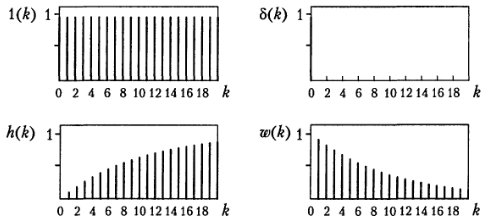
\includegraphics[width=0.5\linewidth]{images/input/kt.png}
    \caption{Caption}
    \label{fig:my_label}
\end{figure}

При нулевых начальных условиях системы:
\begin{equation}
    h(0) = \dots = h(-n+1) = 0, w(0) =  \dots = w(-n+1) = 0
\end{equation}
Единичная импульсная последовательность:
\begin{equation}
    \mathbf{1}(k) =
    \begin{cases}
    0, k < 0, \\
    1, k \ge 0.
    \end{cases},
    \quad
    h(k) = y(k)|_{y_o(k) = 0, u(k) = \mathbf{1}(k)} = y_{\text{в}}
\end{equation}

Дельта функция:
\begin{equation}
    \mathbf{\delta}(k) =
    \begin{cases}
    0, k \ne 0, \\
    1, k = 0.
    \end{cases},
    \quad
    w(k) = y(k)|_{y_o(k) = 0, u(k) = \mathbf{\delta}(k)} = y_{\text{в}}
\end{equation}

\textbf{Установившаяся составляющая.}
\begin{equation}
    y_{\text{у}} = \cfrac{b_1 + \dots + b_n}{1+a_1 + \dots + a_n} u = K u = W(1) u
\end{equation}
где $K$~--- \textit{статический коэффициент}.

Условие существования статической характеристики:
\begin{equation}
    1+a_1 + \dots + a_n \ne 0
\end{equation}
и система удовлетворяющая этому условию называетя статической.





\subsection{Дискретное преобразование Лапласа (Z-преобразование) дискретных процессов}

В теории импульсных систем для решения разностных уравнений используется дискретное преобразование Лапласа и его модификация~--- дискретное z-преобразование.

Преобразование лапласа для непрерывной и дискретной функций:
\begin{equation}
    X(s) = \int\limits_{0}^{\infty} x(t) e^{-st} dt, \quad  X(s) = T \sum\limits_{k=0}^{\infty} x(kT) e^{-s kT}
\end{equation}

Дискретное преобразование Лапласа, получается путем введением замены:
\begin{equation}
    z^-k = e^{sT} 
    \quad\Rightarrow\quad
    X(z) = T \sum\limits_{k=0}^{\infty} x(kT) z^{-k}
\end{equation}
$x(kT$~--- оригинал решетчатой функции, $X(z)$~--- его изображение, $z$~--- комплексная переменная.

Из теоремы Коши-Адамара следует, что ряд сходится абсолютно вне круга $|z|>R$, где $R = \lim\limits_{k \rightarrow \infty} (|x(kT)|)^{\frac{1}{k}}$.

Для полубесконечной последовательности $\{x(k)\}$ ($x(k) = 0, k < 0$):
\begin{equation}
    x(0), x(1), x(2), \dots
\end{equation}

Ее можно рассматривать как функцию, аргумент которой применает дискретные значения $0,1,2, \dots$. Такие функции называю решетчатыми функциями.

Z- преобразованием последоватьности называют сумму ряда
\begin{equation}
    X(z) = Z\{x(kT)\} = \sum\limits_{k=0}^{\infty} x(kT) z^{-k}.
\end{equation}


Оно лежит в основе метода решения разностных уравнений. Дискретное преобразование Лапласа $X(z)$ отличается от z-преобразования наличием нормирующего множителя $Т$. При анализе дискретных систем z-преобразование позволяет перейти от разностных уравнений к алгебраическим и существенно упростить анализ динамики дискретных систем.

Для обратного перехода от изображения к оригиналу (для нахождения исходной решетчатой функции по ее изображению) используется обратное z-преобразование:
\begin{equation}
    x(kT) = \cfrac{1}{2 \pi j} \oint X(z) z^{k-1} dz
\end{equation}

Корни $s_i$ характеристического полинома непрерывной системы связаны с корнями $z_i$ характеристического полинома эквивалентной дискретной системы соотношением
\begin{equation}
    z_i = e^{p_iT}
\end{equation}
Взаимно-однозначное соответствие корней непрерывной и эквивалентной дискретной систем выполняется только при интервале дискретизации, удовлетворяющем теореме Котельникова-Шеннона.

Важно, что все существующие изображения имеют общую область сходимости --- круг некоторого радиуса $R_{min}$ в комплексной плоскости $\xi$ и область вне круга радиуса $1/ R_{min}$ в плоскости $z$.

\textcolor{blue}{Свойства z-преобразования}.

\begin{enumerate}
    \item Линейность. Для любых $a, b$
    \begin{equation}
        Z\{a x(k) + b y(k)\} = a X(z) + b Y(z)
    \end{equation}
    
    \item Начальное значение последовательности может быть вычислено как
    \begin{equation}
        x(0) = \lim\limits_{z \rightarrow \infty} X(z)
    \end{equation}
    
    \item Конечное значение. Если функция $(1-z^{-1}) X(z)$ не имеет полюсов в области $|z| \ge 1$ и конечное значение последовательности $\{x(k)\}$ существует, оно может быть вычислено как
    \begin{equation}
        \lim\limits_{k \rightarrow \infty} x(k) = \lim\limits_{z \rightarrow \infty} (1-z^{-1}) X(z)
    \end{equation}
    
    \item Обратные сдвиг.
    
    Последовательность $\{x(k-m)\}$, запаздывающую на $m > 0$ такток по отношению к исходной последовательности
    \begin{equation}
        Z\{x(k-m)\} = z^{-m} X(z)
    \end{equation}
    
    \item Сдвиг вперед
    \begin{equation}
        Z\{x(k+m)\} = z^{m} \Bigg[ X(z) - \sum\limits_{i=0}^{m-1} x(i) z^{-i} \Bigg]        
    \end{equation}
    
    \item Свертка решетчатых функций $\{x(k)\}, \{y(k)\}$
    \begin{equation}
        g(k) = \sum\limits_{m=0}^{k} x(m) y(k-m) = \sum\limits_{m=0}^{k} x(k-m) y(m)
    \end{equation}
    имеет изображение, равное произведению этих функций
    \begin{equation}
        Z\{g(k)\} = X(z) Y(z)
    \end{equation}
\end{enumerate}
\subsection{Передаточные функции и матрицы дискретных систем и объектов и их вычисление на основе структурного представления}

ПФ~--- отношение дискретного преобразования Лапласа входной переменной к выходной при нулевых начальных условиях:
\begin{equation}
    W(z) = \cfrac{Y(z)}{X(z)}
\end{equation}

Передаточная матрица:
\begin{gather}
    \text{for} z\{x(k)\} = X(z), \quad z\{u(k)\} = U(z), \quad z\{y(k)\} = Y(z), \\
    \begin{cases}
        x(k+1) = A x(k) + B u(k),\\
        y(k) = C x(k),
    \end{cases}
    \quad\Rightarrow\quad
    \begin{cases}
        z X(z) = A X(z) + B U(z),\\
        Y(z) = C X(z),
    \end{cases}
\end{gather}
Отсюда, получим предаточную матрицу:
\begin{gather}
    Y(z) = C(z I - A)^{-1} B \cdot U(z)
    \quad\Rightarrow\quad
    W(z) = C(z I - A)^{-1} B
\end{gather}
где
\begin{gather}
    W(z) = \Big[ W_{ij}(z) \Big], i=\overline{1,n}, j=\overline{1,n}
\end{gather}
где $W_{ij}$~--- связывает i-ый вход с j-ым выходом.

Пример:
\begin{equation}
    Y(z) = \cfrac{W_1 W_2}{1+W_1 W_2} G(z) + \cfrac{W_2}{1+W_1 W_2} F(z),
\end{equation}
где $G(z)$~--- изображение входа, $F(z)$~--- изображение помехи.
\subsection{Структурные свойства линейных непрерывных и дискретных ОУ: управляемость и 	наблюдаемость}
\subsection{Критерии управляемости и наблюдаемости непрерывных 	и дискретных ОУ}


\textbf{Управляемость}~--- это структурное свойство объекта (модели), означающее что что перезод из любого состояния системы в любое другое систояние может быть достигнуто приложением некоторого  ограниченного управляющего воздействия.

С. полностью управляема, если для любых $t >= 0$ и $x_f \in \mathcal{R}$ существует такое $t_f >= t_0)$ и ограниченное управляющее воздействие $u(t), t \in [t_0, t_f]$ такое, что для $x(t_0) = x_0$ выполняется $x(t_f) = x_f$.

Матрица управляемости:
\begin{equation}
    U = [B, AB, \dots,A^{n-1} B]
\end{equation}

Критерий управляемости:
\begin{enumerate}
    \item Линейная система полностью управляемая тогда и только тогда, когда (если $rank(U) = n$, $n$ порядок системы).
    \begin{equation}
        \det(U) \ne 0.
    \end{equation}

    \item C. полностью управляема тогда и только тогда, когда она может быть преобразована к канонической управляемой форме.
\end{enumerate}
Свойство управляемости не зависит от выходной переменной.

\textbf{Наблюдаемость}~--- свойство системы, при котором ее переменные состояния могут быть однозначно определены по выходной переменной y.

Система нызвается полностью наблюдаемой, если для любых $t_0\ge 0$ существует $t_1 > t_0$ такое, что выходной переменной
\begin{equation}
    y = y(t), t \in [t_0, t_1]
\end{equation}
полученной для входного сигнала $u(t)$, соответствуйте единственное значение $x(t_0) = x_0$.

Матрица наблюдаемости:
\begin{equation}
    Q = 
    \begin{bmatrix}
        C\\
        CA\\
        \cdots\\
        C A^{n-1}
    \end{bmatrix}
\end{equation}

Линейная система полностью наблюдаема, если $rank (Q) = n$, т.е
\begin{equation}
    \det Q \ne 0.
\end{equation}
\subsection{Понятие разностных уравнений и способы их решений}

Для объекта:
\begin{equation}
    \begin{cases}
        x(k+1) = A x(k) + Bu(k),\\
        y(k) = C x(k).
    \end{cases}
\end{equation}

\textbf{Аналитическое решение} разностного уравнения в форме ВСВ:
\begin{gather}
    x(1) = A x(0) + B u(0),\\
    x(2) = A^{2} x(0) + A B u(0) + B u(1),\\
    x(3) = A^3 x(0) + A^2 B u(0) + A B u(1) + B u(2),\\
    x(k) = \underbrace{A^k x(0)}_{\text{св. сост-ая}} + 
    \underbrace{\sum\limits_{i=0}^{k} A^{k-1-i} B u(i)}_{\text{в. сост-ая}}
\end{gather}

\textbf{Аналитическое решение} разностного уравнения в рекуррентном виде:
\begin{equation}
    a_0 y(k+n) + a_1 y(k+n-1) +\dots+ a_n y(k) = b_1 u(k+n-1) +\dots+ b_n u(k)
\end{equation}

Форма представления моделей дает простой путь для получения рекуррентного решения, т. е. процедуры нахождения текущих значений $y(k)$ по известным значениям функций у и u в предшествующие моменты дискретного времени k. Подставляя в разностное уравнение $k+n=k$ (или $n= 0$) запишем:
\begin{equation}
    y(k) = -a_1 y(k-1) -\dots- a_n y(k) + b_1 u(k-1) + b_2 u(k-2) + \dots + b_n u(0)
\end{equation}
\begin{equation}
    \sum\limits_{i=0}^{n} a_i y (k+n-i) = \sum\limits_{j=0}^{k} b_j u(k+j)
\end{equation}
Сдвиг входной переменно k должен быть не больше сдвига n: $k \le n$~--- уловие физической реализуемости.

Пример:

Характеристическое уравнение системы:
\begin{equation}
    z^2 + a_{n-1} z^{n-1} + \dots + a_q z + a_o = 0
\end{equation}

\begin{equation}
    y(k) = \sum\limits_{i=1}^{n} C_i z_i^k + y_{\text{в}}(k)
\end{equation}

Найдем вынужденную составляющую из
\begin{equation}
    \sum\limits_{i=0}^{n} a_i y_{\text{в}}(k+i) = \sum\limits_{j=0}^{k} b_j u(k+j)
\end{equation}
Затем, найдем неопределенные коэффициенты $C_i$ из условия, что общее решения для n-1 интервала должно быть равно начальным условиям $y(0),y(1), \dots, y(n)$.
\begin{gather}
    \sum\limits_{i=0}^{n} C_i +  y_{\text{в}}(0) = y(0),\\
    \sum\limits_{i=0}^{n} C_i z_i+  y_{\text{в}}(1) = y(1),\\
    \sum\limits_{i=0}^{n} C_i z_y^2+  y_{\text{в}}(2) = y(2),\\
    \sum\limits_{i=0}^{n} C_i z_y^n +  y_{\text{в}}(n) = y(n).
\end{gather}




\section*{\centering РАЗДЕЛ II. Анализ устойчивости линейных непрерывных и дискретных систем}
\subsection{Понятие 	устойчивости. Виды устойчивости: 	устойчивость по Ляпунову, асимптотическая 	устойчивость, экспоненциальная устойчивость, качественная экспоненциальная 	устойчивость непрерывных и дискретных 	систем}


\textcolor{blue}{\textbf{Устойчивость} это}~--- способность динамической системы возвращаться в исходное положение равновесия после окончания действия внешних возмущений.

В классической теории устойчивости исследуется не устойчивость системы как таковой, а устойчивость ее так называемого невозмущенного движения. Для линейных систем с точки зрения устойчивости не имеет значения, какое их движение принимается в качестве невозмущенного.

Некоторые справедливые (Бессекерский, c. 119) замечания:
\begin{enumerate}
    \item Устойчивость невозмущенного движения не зависит от того, какое движение
системы принято в качестве невозмущенного.
    \item Певозмущенное движение системы устойчиво, если устойчиво ее свободное
движение.
    \item Устойчивость невозмущенного движения не зависит от вида и характера из-
менения внешних (задающего и возмущающих) воздействий. Этот вывод ба-
зируется на двух предыдущих.
\end{enumerate}

\textit{Теорема Ляпунова}:
Если для уравнений возмущенного движения можно найти знакоопределенную функцию $V$, производная $\dot V$ которой в силу этих уравнений была бы или знакопостоянной функцией противоположного знака с $V$, или тождественно равной нулю, то невозмущенное движение $x=0$ устойчиво.


\textcolor{blue}{\textbf{Виды устойчивости}} (для дискретных все тоже самое только для дискретного времени):
\begin{enumerate}
    \item \textcolor{blue}{\textit{устойчивость по Ляпунову}}.
    
    Система устойчива по Ляпунову, если для любого $\epsilon > 0$, найдется $\delta(\epsilon) > 0$ такое, что для всех начальных условий удовлетворяющих $|x_0| < \delta$ и любого $t>0$, выполняется $|x(t,x_0)| < \epsilon$.
    
    Если это условие не вполняется, то система называется неустойчивой.
    
    Определение предусматривает, что траектории $x(t,x_0)$ начинающиеся в некторой малой $\delta$-окрестности положения равновесия, не покидают заданную $\epsilon$-окрестность.
    
    \item \textcolor{blue}{\textit{асимптотическая устойчивость}}.
    
    Система называется асимптотически устойчивой, если
    \begin{enumerate}
        \item она устойчива по Ляпунову;
        \item выполняется условие аттрактивности (притяжения) положения равновесия:
        \begin{equation}
            \lim\limits_{t \rightarrow \infty} x(t, x_0) = 0
        \end{equation}
    \end{enumerate}
    Из асимптотической устойчивости следует устойчивость по Ляпунову.
    
    Определение предусматривает, что положение равновесия обладает притягивающими свойствами, т.е. с течением времени приближвается к положению равновесия $x^*=0$. Но определить время схождения нельзя.
    
    \textcolor{green}{
        \textbf{Дискретная система}
        \begin{equation}
            \begin{cases}
                x(k+1) = A x(k)\\
                y(k) = C x(k)
            \end{cases}
        \end{equation}
        асимптотическая устойчива, если $\lim\limits_{k \rightarrow \infty} |x(k)| = 0$.
    }
    
    
    \item \textcolor{blue}{\textit{экспоненциальная устойчивость}}.
    
    Система экспоненциально устойчива, если найдутся таке числа $c>0, \alpha>0$, что для любых $t \ge 0$, вполняется:
    \begin{equation}
        x(t, x_0) \le c e^{-\alpha t} |x_0|.
    \end{equation}
    
    Отсюда видно, что все траектории, начинающиеся в произвольной $\Delta_0$-окрестности, т.е. $|x_0| \le \Delta_0$, экспоненциально затухают~--- находятся в каждый момент времени $t$ в пределах сужающейся области:
    \begin{equation}
        |x| < x_m(t) = c \Delta_o e^{-\alpha t}.
    \end{equation}
    Фунция $x_m(t)$ ограничивающая сверху текущие значения нормы вектора состояния, называется \textit{мажорантой}.
        
    При определенных условиях экспоненциальная и асимптотическая устойчивости эквивалентны.
            
    \item \textcolor{blue}{\textit{качественная экспоненциальная устойчивость}}.
    
    Система КЭ устойчива для любых траеткорий движения системы и начальных условий, найдется такие $r>0, \beta: \beta + r < 0$, что для любых $t \ge 0$ выполняется неравенство:
    \begin{equation}
        || x(t) - e^{\beta t} x(0) || \le \rho (e^{(\beta - r) t} -e^{\beta t}) ||x(0)||,
    \end{equation}
    где $\rho > 0$.
    
    

\end{enumerate}
\subsection{Корневые 	условия устойчивости непрерывных и 	дискретных систем}

\textcolor{blue}{\textbf{Корневые критерии устойчивости}} связывают понятие устойчивости с размещением корней на комплексной плоскости:
\begin{enumerate}
    \item Для непрерывных систем: 
    \begin{enumerate}
        \item устойчива~--- все корни в левой полуплоскости;
        \item устойчива по Ляпунову~--- один корень на границе устойчивости;
        \item неустойчива~--- хотябы один корень в правой полуплоскости.
    \end{enumerate}
    
    \item Для дискретных систем (могут быть эелементарно выведены из теории непрерывных систем, учитывая связь корней Н. и Д. систем $z_i = e^{T p_i}$):
    \begin{enumerate}
        \item устойчива~--- все корни строго внутри единичной окружности;
        \item устойчива по Ляпунову~--- один корень на окружности;
        \item неустойчива~--- хотябы один корень вне единичной окружности.
    \end{enumerate}
\end{enumerate}

Критерии:
\begin{enumerate}
    \item Система асимптотически устойчива тогда и только тогда, когда выполняется условие:
    
    Звенья: апериодической (I и II), колебательное.
    \begin{equation}
        Re p_i < 0, \quad i = \overline{1,n}.
    \end{equation}
    
    \item Система устойчива по Ляпунову, если выполняется одно из условий:
        \begin{enumerate}
            \item Апериодическая граница устойчивости (наличие одного вещественного корная на границе устойчивости (мнимой оси)): 
    
            Звенья: Интегратор.
            \begin{equation}
                \begin{cases}
                    \Re p_i < 0, \quad i = \overline{1, n-1}, \\
                    p_n = 0
                \end{cases}
            \end{equation}
            
            \textcolor{green}{
                \textbf{Дискретная полностью наблюдаемая система асимпототический устойчива тогда и только тогда, когда выполняется условие}:
                \begin{equation}
                    |z_i| = |\lambda_i\{A\}| < 1, \quad i = \overline{1,n}.
                \end{equation}
            }
    
            \item Колебательна граница устойчивости (наличие двух комплексно-сопряженных корней на мнимой оси):
            
            Звенья: консервативное (генератор).
            \begin{equation}
                \begin{cases}
                    \Re p_i < 0, \quad i = \overline{1, n-2}, \\
                    \Re p_{n-1, n} = 0, \quad \Im p_{n-1, n} \ne 0.
                \end{cases}
            \end{equation}
        \end{enumerate}
        
    \item Система неустойчива, если хотябы один полюс такой, что
    \begin{equation}
        \Re p_i > 0.
    \end{equation}
\end{enumerate}
\subsection{Алгебраические критерии устойчивости непрерывных систем}
\subsection{Методы Ляпунова в исследовании устойчивости непрерывных и дискретных систем}

Критерии устойчивости позволяют осуществить анализ системы, не прибегая к определениям устойчивость (где нужно было бы анализировать все возможные переходные прцессы), т.е. на основании косвенных признаков устойчивости, связанных со свойствами математических моделей.

Для автономной системы, решения для которой представляются в виде:
\begin{gather}\label{solves}
    x(t) e^{At}x_0,
    \quad
    y(t) = C^T e^{At} x_0 = \sum\limits_{i=1}^{n} C_i e^{p_i t},
\end{gather}
где $C_i$~--- коэффициенты, зависящие от НУ, $p_i$~--- полюсы системы, или корни характеристическогоого полинома:
\begin{equation}
    a(p) = \det(pI - A) = p^n + a_1 p^{n-1} + \dots + a_n.
\end{equation}

Выражения~\eqref{solves} плказывают, что свойства преходных процессов в целом определяются свойствами компоненты $e^{At}$, которые зависят от полюсов системы (корней характеристического полинома), или, что тоже самое, от собственных чисел матрицы $A$. 

\begin{enumerate}
    \item \textcolor{blue}{Метод Гурвица}
    
    \textbf{Теорема Стодолы}: если система устойчива, то коэффициенты характеристического полинома (ХП) строго положительны (обратное верно только для систем 1 и 2 порядка (\textcolor{gray}{чем и обусловлены более сложные условия в критерии Гурвица и подобных})).
    
    \textbf{Критерий Гурвица}:
    \begin{enumerate}
        \item Система с характеричтическим уравнением устойчива тогда и только тогда, когда все определители $\Delta_i$ матрицы Гурвица строго положительны: $\Delta_i > 0, i=\overline{1,n}$.
        \item Система нейтрально устойчива, елси выполняется одно из условий:
        \begin{enumerate}
            \item Апериодическая граница устойчивости (итегратор)
            \begin{equation}
                \begin{cases}
                    \Delta_i > 0, \quad i=\overline{1, n-1}, \\
                    \Delta_n = \Delta_{n-1} a_n = 0,
                \end{cases}
            \end{equation}
            \item Колебательная граница устойчивости (консервативное звено)
            \begin{equation}
                \begin{cases}
                    \Delta_i > 0, \quad i=\overline{1, n-2}, \\
                    \Delta_{n-1} = 0, \\
                    a_n > 0.
                \end{cases}
            \end{equation}
        \end{enumerate}
    \end{enumerate}
    
    Матрица гурвица:
    \begin{equation}
        \begin{bmatrix}
            a_1 & a_2 & a_3 &\cdots & 0 & 0 \\
            a_0 & a_2 & a_3 &\cdots & 0 & 0 \\
            0 & a_1 & a_3 &\cdots & 0 & 0 \\
            \cdots & \cdots & \cdots & \cdots & \cdots & \cdots \\
            0 & 0 & 0 &\cdots & a_{n-1} & 0 \\
            0 & 0 & 0 &\cdots & a_{n-2} & a_n
        \end{bmatrix}
    \end{equation}
    
    Определители Гурвица~--- главные диагональные миноры матрица М:
    \begin{equation}
        \Delta_1 = a_1, \quad
        \Delta_2 = 
        \begin{bmatrix}
            a_1 & a_3 \\
            a_0 & a_2
        \end{bmatrix}
        = a_1 a_2 - a_0 a_3, \quad
        \cdots, \quad
        \Delta_n = |M| = a_n \Delta_{n-1}.
    \end{equation}
    
    \item \textcolor{blue}{Корневые критерии} \textcolor{red}{(см. предыдущий вопрос про корневые критерии)}
    \begin{equation}
        \cdots
    \end{equation}
    
    \item \textcolor{blue}{Метод Ляпунова}
    
    Матрица A назвается устойчивой или гурвицевой, если выполняется условие $\Re(\lambda_i\{A\}) < 0, i = \overline{1,n}$.
    
    \textbf{Лемма Ляпунова.} Матрица A устойчива тогда и только тогда, когда для любых матриц $Q = Q^T > 0$ уравнение имеет положительно определенное решение $P>0$:
    \begin{equation}
        A^T P + PA = - Q
    \end{equation}
    где $Q = Q^T >0$.
    
     Т.о. существование решения уравнения Ляпунова обеспеивает устойчивость матрицаы A (асимптотическая устойчивость).
     
     Для оценци качества сходимости ПП устойчивой системы рассматривается следующее выражение:
     \begin{equation}\label{eqL}
         A^T P + PA = -Q - 2 \alpha P
     \end{equation}
    
    \textbf{Свойство.} Матрица A удовлетворяет условию
    \begin{equation}
        \Re(\lambda_i\{A\}) < -\alpha, i = \overline{1,n}
    \end{equation}
    тогда и только тогда, когда уравнение~\eqref{eqL} для любых $Q=Q^T >0$ имеет положительно определеное решение $P>0$.
    
    Это условие при $\alpha > 0$ означает, что полюсы системы, смещены влево от границы устойчивости на велечину, превышающую значение $\alpha$, что предполагает асимптотическую устойчивость с \textit{запасом устойчивости}.
\end{enumerate}

\subsection{Частотные критерии устойчивости непрерывных систем}

\textcolor{blue}{\textbf{Критерий Найквиста}} позволяет определить устойчивость замкнутой системы, построив частотную характеристику разомкнутой системы.

Чтобы система в замкнутом состоянии была устойчивой необходимо и достаточно, чтобы при изменении $\oemga$ от $-\infty$ до $\infty$  годограф разомкнутой системы $W(j \omega)$ (АФХ), поворачиваясь вокруг начала координат по часовой стрелке, охватил точку $(−1,j0)$ столько раз, сколько корней в правой полуплоскости содержит знаменатель $W(j \omega)$.

Примечания:
\begin{enumerate}
    \item Если корней в правой полуплоскости нет, то годограф $W(j\omega)$ не должен охватить точку $(−1,j0)$.
    \item Неустойчивая система в разомкнутом состоянии может быть устойчивой в замкнутом состоянии. И наоборот.
    \item Годограф $W(j\omega)$ всегда начинается на оси "$+1$". Но при порядке астатизма равном r, по причине устремления $W(j\oemga)$ к $\infty$ (при $\omega \rightarrow$), видимая часть годографа появляется только в квадранте r, отсчитанном по часовой стрелке.
\end{enumerate}

Свойства годографа Найквиста
\begin{enumerate}
    \item Годограф Найквиста спиралевиден. При $\oemga \rightarrow \infty$ годограф $W(j\omega)\rightarrow 0$, т.к. нет безынерционных систем.
    \item Годограф статических САР начинается из точки на вещественной оси.
    \item Для положительных и отрицательных частот годографы зеркально симметричны относительно оси "+1". Наличие корней на границе устойчивости приводит к устремлению годографа в $\infty$ и приращению его фазы на $-180^o$.
\end{enumerate}

Для определения устойчивости по критерию Найквиста можно строить не АФХ, а ЛАЧХ и ЛФЧХ разомкнутой системы. Чтобы замкнутая система была устойчива, необходимо и достаточно, чтобы сдвиг фазы на частоте единичного усиления разомкнутой системы $W(j \omega)$ не достигал значения $-180^o$.
Если система условно устойчивая, то при модулях больших единицы, фазовый сдвиг может достигать значения $-180^o$ четное число раз.

\textcolor{blue}{\textbf{Критерий устойчивости Михайлова}}.

Чтобы все корни ХУ имели отрицательные вещественные части, необходимо чтобы после подстановки частоты в соответствующий характеристический полином $D(s)$ полное приращение его фазы при изменении $\oemga$ от $0$ до $\infty$ составляло $n \pi / 2$, где $n$~--- степень полинома $D(s)$. При этом характеристический полином опишет в комплексной плоскости кривую~--- "годограф Михайлова".

\begin{enumerate}
    \item Пусть $s_i=\alpha$~--- вещественный положительный корень. Тогда годограф соответствующего линейного множителя $(j\omega - \alpha)$ при изменении $\omega$ от 0 до $\infty$ повернется на угол $-\pi/2$.

    \item Пусть $s_i=-\alpha$~--- вещественный отрицательный корень. Тогда годограф соответствующего линейного множителя $(j\omega + \alpha)$ при изменении $\omega$ от 0 до $\infty$ повернется на угол $\pi/2$.

    \item Пусть $s_{i; i+1}= \alpha \pm j\beta$~--- сопряженные корни с положительной вещественной частью. Тогда годографы соответствующих линейных множителей $(j\omega−\alpha−j\beta)(j\omega−\alpha+j\beta)$ при изменении $\omega$ от 0 до $\infty$ повернутся на углы $-\pi/2+\gamma$, и $\pi/2-\gamma$. Вектор, соответствующий произведению двух сомножителей, повернется на угол равный $-\pi$.

    \item Пусть $s_{i; i+1}=-\alpha \pmj\beta$~--- сопряженные корни с отрицательной вещественной частью. Тогда годографы соответствующих линейных множителей $(j\omega+\alpha-j\beta)(j\omega+\alpha+j\beta)$ при изменении $\omega$ от 0 до $\infty$ повернутся на углы $\pi/2−\gamma$, и $\pi/2+\gamma$. Вектор, соответствующий произведению двух сомножителей, повернется на угол равный $\pi$.
\end{enumerate}


Резюме: Если ХУ имеет $l$ корней с положительной вещественной частью, то угол поворота годографа $D(j\omega)$ при изменении $\omega$ от 0 до $\infty$ составит:
\begin{equation}
    \psi= - l \pi 2+ (n-l) \pi 2=n \pi 2-l \pi,    
\end{equation}
где: $n$~--- порядок ХУ.

Свойства годографа Михайлова
\begin{enumerate}
    \item Годограф всегда спиралевиден.
    \item При $\omega=0$, будет $\psi=0$. Следовательно, годограф начинается с точки на оси "+1".
    \item Поскольку при $\omega\rightarrow\infty, K(j\omega)\rightarrow 0$ (нет безынерционных систем), годограф уходит в бесконечность.
    \item При четном n, годограф стремится к $\infty$ параллельно оси "+1"; при нечетном n, годограф стремится к $\infty$ параллельно оси "+j".
\end{enumerate}

Определение типа границы устойчивости по виду годографа Михайлова
\begin{enumerate}
    \item Астатизм первого порядка~--- "апериодическая" граница устойчивости.
    \item Астатизм второго порядка~--- "апериодическая" граница устойчивости.
    \item "Колебательная" граница устойчивости.
    \item Граница устойчивости типа "бесконечный корень".
\end{enumerate}

\subsection{Степень устойчивости, запас устойчивости по 	фазе и амплитуде, их определение с помощью амплитудно-фазовых частотных характеристик или ЛАЧХ и ФЧХ непрерывной 	системы}

В условиях эксплуатации параметры системы по тем или иным причинам могут меняться в определенных пределах (старение, температурные колебания и т.п.). Эти колебания параметров могут привести к потере устойчивости системы, если она работает вблизи границы устойчивости. Поэтому стремятся спроектировать САУ так, чтобы она работала вдали от границы устойчивости. Степень этого удаления называют запасом устойчивости.

Согласно критерия Найквиста, чем дальше АФЧХ от критической точки (-1, j0), тем больше запас устойчивости. Различают запасы устойчивости по модулю и по фазе.

Запас устойчивости по модулю характеризует удаление годографа АФЧХ разомкнутой САУ от критической точки в направлении вещественной оси и определяется расстоянием h от критической точки до точки пересечения годографом оси абсцисс (левый рисунок).

Запас устойчивости по фазе характеризует удаление годографа от критической точки по дуге окружности единичного радиуса и определяется углом  между отрицательным направлением вещественной полуоси и лучом, проведенным из начала координат в точку пересечения годографа с единичной окружностью.

\begin{figure}[!h]
    \centering
    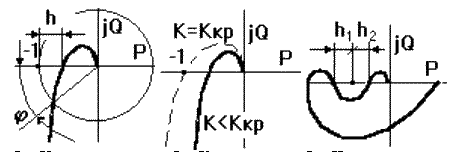
\includegraphics[width=0.5\textwidth]{images/stab.png}
    \caption{Поясняющие рисунки}
    \label{fig:stubs}
\end{figure}

Как уже отмечалось, с ростом коэффициента передачи разомкнутой САУ растет модуль каждой точки АФЧХ и при некотором значении K = Kкр АФЧХ пройдет через критическую точку (средний рисунок) и попадет на границу устойчивости, а при K > Kкр замкнутая САУ станет неустойчива. Однако в случае “клювообразных” АФЧХ (получаются из-за наличия внутренних обратных связей) не только увеличение, но и уменьшение K может привести к потере устойчивости замкнутых САУ (правый рисунок). В этом случае запас устойчивости определяется двумя отрезками h1 и h2, заключенными между критической точкой и АФЧХ.

Обычно при создании САУ задаются требуемыми запасами устойчивости h и, за пределы которых она выходить не должна. Эти пределы выставляются в виде сектора, вычерчиваемого вокруг критической точки, в который АФЧХ разомкнутой САУ входить не должна.





\section*{\centering РАЗДЕЛ III. Показатели качества непрерывных и дискретных систем}

\subsection{ Показатели качества переходных процессов непрерывных и дискретных систем, вводимые по 	переходной функции}

Переходный процесс — в теории систем представляет реакцию динамической системы на приложенное к ней внешнее воздействие с момента приложения этого воздействия до некоторого установившегося состояния. Изучение переходных процессов — важный шаг в процессе анализа динамических свойств и качества рассматриваемой системы. Примерами внешнего воздействия могут быть дельта-импульс, скачок или синусоида.

Прямые показатели качества: время переходного процесса и перерегулирование.

ВПП~--- время, необходимое выходному сигналу системы для того, чтобы приблизиться к своему установившемуся значению. Обычно предел такого приближения составляет $\Delta = 1-10$ процентов.
\begin{equation}
    t_{\text{п}} = min \{ T_{\text{п}}: (h(t) - h_{\text{уст.}}) \le \Delta, t \ge T_{\text{п}} \},
    \quad
    \Delta = 0.05 h_{\text{уст}}
\end{equation}

Перерегулирование (определяется величиной первого выброса) — отношение разности максимального значения переходной характеристики и её установившегося значения к величине установившегося значения. Измеряется обычно в процентах.

\begin{equation}
    \sigma = \cfrac{h_{max} - h_{\text{уст}}}{h_{\text{уст}}} \cdot 100 \%
\end{equation}

Все вышеописанное справедливо и для дискретный систем.
\subsection{Коэффициенты ошибок по задающему и возмущающему воздействиям и их вычисление. Статизм и астатизм непрерывных систем}
\begin{enumerate}
    \item \textbf{По задающему воздействию}.
    
    Коэффициенты ошибок позволяют вычислять установившиееся значение ошибки относительно задающего воздействия на основе разложения задающего воздействия в бесконечнй ряд по производным задающего воздействия.
    
    ПФ по ошибке
    \begin{equation}
        \Phi_e(s) = \cfrac{E(s)}{G(s)} = \cfrac{1}{1 + W(s)} \quad
        E(s) = \Phi_e(s) G(s)
    \end{equation}
    
    Разложив ошибку в ряд Тейлора в окресности $s=0$
    \begin{equation}
        E(s) = (c_0 + c_1 s + \cfrac{c_2 s^2}{2!} + \dots + \cfrac{c_k s^k}{k!}) G(s)
    \end{equation}
    где $c_i$~--- коэффициенты разложения в ряд Тейлора (коэффициенты ошибок).
    
    \begin{equation}
        e_{\text{уст}} (t) = \sum\limints_{i=0}^{p} \cfrac{c_i}{i!} \cdot \cfrac{d^i g(i)}{d t^i} 
        \quad
        c_0 = [\Phi_e(s)]_{s=0},
        \quad
        \cfrac{c_i}{i!} = [\cfrac{d^i \Phi_e(s)}{d s^i}]_{s=0}
    \end{equation}
    
    \item Статическая система
    
    Если коэффициент ошибок $c_0 \ne 0$, то система статическая отностельно задающего воздействия.
    \begin{enumerate}
        \item Для 
            \begin{equation}
                g(t) = g_0 = const \quad
                e_{\text{уст}} = c_0 g_0
            \end{equation}
            
            Статическая система отрабатывает постоянное воздействие с постоянной ошибкой.

        \item Для
            \begin{equation}
                g(t) = g_1 t 
                \quad
                e_{\text{уст}} = c_0 g_1 t + c_1 g_1
            \end{equation}
            
            Статическая система воздействия с постоянной скоростью в установившемся режиме отрабатывает с бесконечной ошибкой (причем ошибка растет в бесконечность линейно).
    \end{enumerate}

    \item Система с астатизмом относительно задающего воздействия
    
    I порядок астатизма:
    \begin{equation}
        c_0 = 0, \quad c_1 \ne 0
    \end{equation}

    \begin{enumerate}
        \item Постоянное входное воздействие
        \begin{equation}
            g(t) = g_0 = const
            \quad
            e_{\text{уст}} = \underbrace{c_0}_{=0} g_0 \textcolor{gray}{(= 0)}
        \end{equation}
        \item Нарастающее входное воздействие
        \begin{equation}
            g(t) = g_1 t \quad
            e_{\text{уст}} = \underbrace{c_0}_{=0} g_1 t + c_1 g_1 = c_1 g_1
        \end{equation}
        Добротность по скорости системы с астатизмом I порядка [$c^{-1}$]
        \begin{equation}
            \cfrac{1}{c_1} = \cfrac{g_1}{e_{\text{уст}}}
        \end{equation}
    \end{enumerate}

    II порядок астатизма:
    \begin{equation}
        c_0 = 0, \quad c_1 = 0, \quad c_2 \ne 0
    \end{equation}
    
    \begin{enumerate}
        \item
        \begin{equation}
            g(t) = g_0 = const \quad
            e_{\text{уст}} = c_0 g_0 + c_1 \cfrac{dg_0}{dt} + \cfrac{c_2}{2} \cfrac{d^2 g_0}{dt^2} + \dots = c_0 g_0 = 0
        \end{equation}
        \item 
        \begin{equation}
            g(t) = g_1 t, \quad
            e = 0, \quad
            \cfrac{dg(t)}{dt} = g_1, \quad
            \cfrac{d^2g(t)}{dt^2} = 0
        \end{equation}
        \item 
        \begin{equation}
            g(t) = \cfrac{g_2}{2} t^2, \quad
            e_{\text{уст}} = \cfrac{c_2}{2} g_2 \quad\Rightarrow\quad
        \end{equation}
        Добротность по ускорению
        \begin{equation}
            \Rightarrow\quad
            \cfrac{g_2}{e} = \Big(\cfrac{c_2}{2}\Big)^{-1}
        \end{equation}
    \end{enumerate}


\end{enumerate}

\subsection{Точность непрерывных систем в типовых режимах}
\subsection{Способы	повышения точностных характеристик 	систем}

Поведение невозмущенной замкнутой системы $y(t) = \Phi(s) y^* (t)$ для различных типов задающего воздействия 
\begin{equation}
    y^* (t) = y_0^* + y_1^* t + y_2^* t^2 + \dots, \quad
    y_i^* (t) = \cfrac{y^* (0)}{i!} = const
\end{equation}
В зависимости от $y_i^*$ различают режимы:
\begin{enumerate}
    \item стационарный (стабилизация) $y^*=y^*_0$
    \item режим движения с постоянной скоростю $y^* = V_0 t$
    \item режим движения с постоянным ускорением $y^* = \cfrac{a_0 t^2}{2}$
\end{enumerate}

Вводятся коэффициенты ошибок для оценки точность
\begin{gather}
    \Phi_0 = \Phi(0) = \cfrac{W(s)}{1 + W(s)}|_{s=0};
    \quad
    \Phi_1 = \Phi'(0) = \cfrac{W'(s)}{(1+ W(s))^2}|_{s=0}
    \quad
    \Phi_2 = \Phi'' (0) = \cfrac{W''(s) (1 + W(s)) - 2 W'(s)}{(1+W(s))^3}|_{s=0}\\
    y_{\text{уст}}(t) = \Phi_0 y^* + \Phi_1 \dot y^* + \cfrac{\Phi_2}{2!} \ddot y^* + \dots\\
    e_{\text{уст}}(t) = (1 - \Phi_0) y^* - \Phi_1 \dot y^* - \cfrac{\Phi_2}{2!} \ddot y^* + \dots
\end{gather}

\begin{enumerate}
    \item В стационарном режиме $y_{\text{уст}} = \Phi_0 y^*$.
Абсолютняа точность и установившаяся ошибка достигается при $\Phi_0 = 1$, что выполняется для астатических систем. Для статическых систем $e_{\text{уст}} = \cfrac{1}{1+k} y^*$. Ошибку можно уменьшить засчет увеличения коэффициента обратной связи.
    
    \item В режиме движения с постоянной скоростью имеет место
    \begin{equation}
        y_{\text{уст}} = \Phi_0 y^* + \Phi_1 V_0 = \Phi_0 V_0 t + \Phi_1 V_0
    \end{equation}
    Абсолютная точность при $\Phi_0 = 1, \Phi_1 = 0$~--- астатизм 2 порядка и выше.
    
    Для астататизма перого порядка $e_{\text{уст}} = \cfrac{1}{k_1} V_0$. Для уменьшения установившейся ошибки увеличивать коэффициенты обратной связи.
    
    Для статического режима~--- с течением времени ошибка неограничено возрастает.
    
    \item В режиме с постоянные ускорением
    \begin{equation}
        y_{\text{уст}} = \Phi_0 y^* + \Phi_1 a_0 V + \cfrac{\Phi_2}{2!} a_0 = \Phi_0 \cfrac{a_0 t^2}{2!} + \Phi_1 a_0 t + \Phi_2 \cfrac{a_0}{2}
    \end{equation}
    Абсолютная точность $\Phi_0=1, \Phi_1 = \Phi_2 = 0$, что выполняется для астатических систем порядка 3 и выше
    
    Для астатизма второго порядка $e_{\text{уст}} = \cfrac{1}{k}a_0$
\end{enumerate}

Повышение точности достигается:
\begin{enumerate}
    \item подключением обратных вязей (замыкание системы).
    \item повышение порядка статизма основного канала с помощбю соответствующих регуляторов (алгоритмов управления)
    \item повышение добротности системы за счет увеличения коэффициентов регуляторов.
\end{enumerate}


\section*{\centering РАЗДЕЛ IV. Методы синтеза непрерывных и дискретных систем на заданные требования к качеству процессов в переходном и установившемся режимах}

\subsection{Общий подход к синтезу непрерывных систем на основе логарифмических частотных характеристик. Типовые желаемые логарифмические амплитудно-частотные характеристики}

Синтез системы
Направленный расчет, имеющий конечной целью отыскание: 1) рациональной структуры системы и 2) установление оптимальных величин параметров отдельных звеньев.
При множестве возможных решений, должен быть выбран критерий оптимизации – цена, точность, надежность, быстродействие, затраты энергии ...

При инженерном синтезе ставятся задачи:

Достижение требуемой точности.
Обеспечение приемлемого характера переходных процессов (задача демпфирования).
Решение первой задачи заключено в выборе средств повышающих точность системы (усилительных, изодромных блоков; каналов КУ; не 1ОС), т.е. фактически вида регулирования.
Решение второй задачи заключено в выборе оптимальных корректирующих средств.


\textbf{Метод логарифмических амплитудных характеристик}
Процесс синтеза включает в себя следующие операции:
\begin{enumerate}
    \item Построение располагаемой ЛАЧХ исходной системы $W_о$, состоящей из регулируемого объекта без регулятора и без корректирующего устройства.
    \item Построение НЧ части желаемой ЛАЧХ на основе предъявленных требований точности.
    \item Определение вида и параметров регулятора $K,K_i,\dots$:
    \begin{gather}
        W_{рег}(s ) = \cfrac{W_{\text{НЧ.ж}}(s)}{W_o(s)}  \\ L_{рег}(\omega)=L_{\text{НЧ.ж}}(\omega)-L_о(\omega).
    \end{gather}
    
    \item Уточнение ВЧ части желаемой ЛАЧХ на основе требований к запасу устойчивости~--- $L_{\text{НЧиВЧ.ж}}(\omega)$.
    \item Определение вида и параметров последовательного корректирующего устройства:
    \begin{gather}
        W_{\text{ПЗкор}} = \cfrac{W_{\text{НЧиВЧ.ж}}}{W_{per}W_о}\\
        L_{\text{ПЗкор}}=L_{\text{НЧиВЧ.ж}}-L_{рег}-L_о.
    \end{gather}
    \item Техническая реализация корректирующих устройств. В случае необходимости~--- перерасчет на эквивалентные параллельное звено или ОС.
    \item Поверочный расчет и построение переходного процесса.
\end{enumerate}


% Процесс синтеза обычно включает в себя следующие операции.
% \begin{enumerate}
%      \item Построение располагаемой ЛАХ. Под располагаемой ЛАХ понимается характеристика исходной системы управления, построенной исходя из требований, предъявляемых к точности режимов стабилизации или слежения, к мощности на выходе системы и т.п. Обычно под исходной системой понимается система, состоящая из управляемого объекта и управляющего устройства и не снабженная необходимыми корректирующими устройствами, обеспечивающими требуемое качество переходного процесса. Исходная система должна быть минимально-фазовой. Это значит, что передаточная функция разомкнутой исходной системы не должна иметь нулей и полюсов, расположенных в правой полуплоскости. Нулями называют корни полинома, стоящего в числителе передаточной функции, а полюсами~--- корни характеристического полинома.
    
%     \item Построение желаемой ЛАХ. Желаемой называют асимптотическую ЛАХ разомкнутой системы, имеющей желаемые (требуемые) статические и динамические свойства. Желаемая ЛАХ состоит из трех основных асимптот: низкочастотной, среднечастотной и высокочастотной. Кроме того, могут быть сопрягающие асимптоты, которые соединяют основные. При построении желаемой ЛАХ необходимо быть уверенным, что вид амплитудной характеристики полностью определяет характер переходных процессов и нет необходимости вводить в рассмотрение фазовую характеристику. Это будет выполняться в случае минимально-фазовых систем.
    
%     \item Определение вида и параметров корректирующего устройства. Наиболее действенным способом придания системе автоматического управления необходимых динамических свойств является введение в нее дополнительного элемента. Он исправляет, корректирует свойства исходной системы и называется корректирующим устройством. Корректирующее устройство включают в систему автоматического управления различным образом. Рассмотрим лишь один способ включения – последовательное включение корректирующего устройства в прямую цепь системы. В этом случае наиболее просто определяется передаточная функция корректирующего устройства, которую обозначим.
    
%     \item Техническая реализация корректирующих устройств. По виду ЛАХ необходимо подобрать схему и параметры корректирующего устройства последовательного типа.
    
%     Применение последовательных корректирующих устройств наиболее удобно в системах, у которых сигнал управления представляет собой напряжение постоянного тока. В этих случаях корректирующее устройство выполняют обычно из пассивных электрических четырехполюсников, обеспечивающих разнообразное преобразование сигнала. Еще больше возможности дают активные (т.е. с дополнительными источниками питания) электрические четырехполюсники постоянного тока.
    
%     \item Поверочный расчет и построение переходного процесса. Нельзя ожидать высокой точности результатов, полученных расчетным путем. Это объясняется прежде всего приближенностью используемого математического описания управляемого объекта и исполнительного элемента. Кроме того, содержат приближения и методы синтеза. Поэтому заключительным этапом расчета должен быть анализ синтезированной системы – определение показателей ее качества. А при физическом осуществлении системы нужна еще ее настройка.
    
%     Указанные обстоятельства не уменьшают значения теоретических расчетов. На основании расчетов выбирается структура корректирующего устройства и ориентировочные значения его параметров. Их отыскание экспериментальным путем значительно сложнее. Вместе с тем моделирование позволяет уточнить выбранные значения параметров.
% \end{enumerate}

\begin{figure}
    \centering
    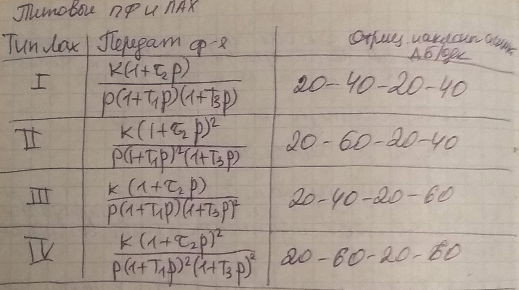
\includegraphics[width=0.7\textwidth]{images/pf.png}
\end{figure}
\subsection{Метод Солодовникова В.В. синтеза непрерывных 	систем}

\subsection{Синтез непрерывных систем с использованием 	показателя колебательности}
\subsection{Модальное 	управление непрерывными и дискретными объектами}

Для объекта
\begin{equation}
    \dot x = A x + bu, \quad y = Cx,
\end{equation}
выбирается П-регулятор (он же модальные) вида
\begin{equation}
    u = - K x
\end{equation}

Такой регулятор вводит обратные свзи по переменным состояния объекта.

Объединение регулятора и объекта дает замкнутую систему:
\begin{equation}
    \dot x = F x = (A - bK) x, \quad y = C x
\end{equation}
где $К$~---матрица строка коэффициентов обратной связи, $F$~--- матрица замкнутой системы.

Выбор коэффициетов обратных связей матрица K обеспечивает получение заданных динамических свойст системы: быстродействие и колебательность.

В соответствиии с методом модального управления устойчивость и заданные показатели качетва достигаются назначением корней характеристического полинома замкнутой системы.

Метод основывается на следующем положении. Если система полностью управляема, то существует единственная матрица обратной свзяи K, обеспечивающая получение заданных значений корней характеристического полинома замкнутой системы.

При отсутствии возмущений, регулятор обеспечивает абсолютную точность стабилизации системы.

Расчет маатрица K:
\begin{enumerate}
    \item По заданным показателям качества находятся корни характеристического полинома $p_i$ и его коэффицинты $a_i$ (например, методом стандартных переходных функций)
    \item Рассчитываются коэффициенты обратной связи K соответствующие канонической управляемой форме объекта
    \begin{equation}
        k_i = a_{ci} - a_i        
    \end{equation}
    \item для обратного перехода от канонической формы к исходной используется матрица подобия
    \begin{equation}
        P = U^* \cdot U^{T}
    \end{equation}
    где $U, U^*$~--- матрицы управляемости исходной и канончиской форм.
    
    Преобразование для перехода 
    \begin{equation}
        K = K^* \cdot P
    \end{equation}
\end{enumerate}


\subsection{Алгоритм 	синтеза модального управления непрерывным 	и дискретными ОУ при полной измеримости его вектора состояния, использующий решение матричного уравнения Сильвестра}

Для объекта
\begin{equation}
    \dot x = A x + bu, \quad y = Cx,
\end{equation}
выбирается П-регулятор (он же модальные) вида
\begin{equation}
    u = - K e \quad e = - x
\end{equation}

Решение задачи:
\begin{enumerate}
    \item Вводится модель ошибок замкнутой системы
    \begin{gather}
        \begin{cases}
            \dot e = F e \\
            v = C e
        \end{cases}
    \end{gather}
    \item Задается эталонная модель ошибор
    \begin{gather}
        \begin{cases}
            \dot \xi = \Gamma \xi, \quad \xi(0) = \xi_0 \\
            \nu = H \xi
        \end{cases}
    \end{gather}
    где $\Gamma$~--- матрица, определяющая требуемые свойства СУ.
    
    ХП матрица $\Gamma$ должен совпадать с требуемым (метод стандартных переходных функций).
    $H$ выбирается из условия полной наблюдаемости пары $\Gamma, H$.
    
    Связь между исходной моделью ошибок и элатонной выражается как
    \begin{equation}
        e = M \xi
    \end{equation}
    
    \item решается систему уравнений включающая уравнение Сильвестра
    \begin{equation}
        \begin{cases}
        M \Gamma - AM = bH \\
        K = - H M^{-1}
        \end{cases}
    \end{equation}
    Все!
    Замечание. Уравнение Сильвестра имеет единственное решение относительно M, если:
    \begin{enumerate}
        \item ОУ полностью управляем (нужно перед всем этим этим проверять)
        \item ЭМ полностью наблюдаема
        \item A и $\Gamma$ не имеют одинаковых корней
    \end{enumerate}
\end{enumerate}



\subsection{Устройства оценки вектора состояния непрерывных 	и дискретных объектов управления при неполной измеримости вектора состояния}

\subsection{Алгоритмы синтеза динамических регуляторов (с устройствами оценки) для непрерывных 	и дискретных объектов управления}
\section{Алгоритм 	синтеза оптимального управления на основе квадратичного функционала 	качества непрерывными объектами при полной измеримости его вектора состояния, использующий решение матричного уравнения Риккати}

Объект и регулятор:
\begin{gather}
    \dot x = A x + b u, \quad y = C x,\\
    u = -K x
\end{gather}

Кватратичный критерий качества:
\begin{equation}
    J = \int\limits_{0}^{t} x^T Q x + r u^2 d\tau
\end{equation}

Сиситема уравнений для нахождения матрицы K
\begin{gather}
    \begin{cases}
        A^T P + PA + Q - P b r^{-1} b^T P = 0\\
        K = r^{-1} b^T P
    \end{cases}
\end{gather}

% 6. .
% 8. .

\end{document}

